\documentclass[conference, onecolumn]{IEEEtran}
\IEEEoverridecommandlockouts
\usepackage{cite}
\usepackage{amsmath,amssymb,amsfonts}
\usepackage{algorithmic}
\usepackage{graphicx}
\usepackage{textcomp}
\usepackage{xcolor}
\usepackage{flushend}
\usepackage{hyperref}
\usepackage{caption}
\def\BibTeX{{\rm B\kern-.05em{\sc i\kern-.025em b}\kern-.08em
    T\kern-.1667em\lower.7ex\hbox{E}\kern-.125emX}}
\begin{document}

\title{Color-Based Object Sorting Machine\\
{\large IOT102t-SE1812, Group 4}}

\author{
Nguyen Tuan Tu, Nguyen Tien Dat, Tran Hoang Tin, Tran Thanh Hoai, and Le The Dung\\
FPT University, Ho Chi Minh Campus, Vietnam\\
\{tuntse181760,
datntse184970,
tinthse185022,hoaittse184132\}@fpt.edu.vn,
\\ dunglt96@fe.edu.vn}
\maketitle

\begin{abstract}
This study aims to develop a Color-Based Object Sorting Machine that enhances sorting processes by automating the classification of objects based on color, improving efficiency and accuracy. The proposed system integrates an Arduino Uno Rev3 microcontroller with key components, including a Bluetooth module, an LCD with I2C interface, a TCS34725 color sensor, a servo motor, and a buzzer. The methodology encompasses both hardware and software design, where the hardware configuration—featuring the TCS34725 color sensor for precise color detection, the servo motor for directing objects, and the buzzer for audible feedback—ensures accurate sorting, while the software component facilitates user-controlled automation through a mobile application. The hardware setup, managed by the Arduino Uno Rev3, provides real-time color recognition and object placement, with the LCD displaying system status and the buzzer signaling process completion or errors. The software, interfacing with the Bluetooth module, allows users to monitor the sorting process, adjust settings, and receive updates via the mobile application. This automation eliminates manual sorting, streamlining tasks in various applications. During testing, the system was evaluated in scenarios such as sorting colored objects in a production line, demonstrating its ability to accurately detect colors, sort efficiently, and provide audible cues via the buzzer. Results indicate reduced sorting errors and enhanced throughput, addressing inefficiencies in traditional methods. The user experience is improved through the intuitive LCD interface and remote control via Bluetooth. In conclusion, the Color-Based Object Sorting Machine leverages IoT technologies to deliver a precise, scalable sorting solution. Its design, centered on the Arduino Uno Rev3 and integrated components, addresses challenges in conventional sorting, offering adaptability for industrial and educational use while contributing to goals of efficiency and automation.
\end{abstract}




\section{Introduction}

Effective object sorting, as a critical process, is essential for optimizing industrial workflows, enhancing automation, and improving efficiency across various applications. It is vital for manufacturing, recycling, quality control, and logistics, where precise categorization of objects based on attributes like color is often required. However, traditional sorting methods, which frequently depend on manual labor or rudimentary mechanical systems, are inefficient, time-consuming, and susceptible to errors. These approaches often lead to inconsistencies, misclassifications, and reduced throughput, resulting in operational bottlenecks and increased costs \cite{smith2019automation}. The growing demand for faster, more accurate sorting solutions is driven by the expansion of industrial automation and the need for sustainable, scalable processes, a challenge recognized globally \cite{patel2022iot, sharma2021automated}.

This demand coincides with a dynamic period of transformation in the Internet of Things (IoT) landscape, which is redefining industrial capabilities worldwide. Today, IoT is no longer an emerging concept but a mature ecosystem, with over 14 billion connected devices reported in 2023 and an increasing focus on edge computing and artificial intelligence integration \cite{iotanalytics2023}. Industries are leveraging IoT to create responsive, data-driven systems that optimize operations in real time, a trend particularly impactful in automation and process management \cite{gupta2020sorting}. In the realm of object sorting, IoT’s ability to connect sensors, devices, and decision-making algorithms offers a compelling solution to the inefficiencies plaguing traditional methods, paving the way for smarter, more adaptable technologies \cite{verma2023iot}.

To address these limitations, there is a strong push to develop and deploy advanced sorting systems harnessing IoT and sensor-based innovations. IoT technologies enable seamless integration of sensors, microcontrollers, and actuators, facilitating real-time data processing, communication, and automated decision-making \cite{patel2022color}. By leveraging IoT, traditional sorting systems can evolve into intelligent solutions that provide precise object detection and classification capabilities. These technologies enhance accuracy in identifying object properties, such as color, and enable rapid sorting, thereby improving productivity and reducing human intervention \cite{singh2022machine}. The Color-Based Object Sorting Machine exemplifies an innovative application of IoT in automated sorting. This system is designed to classify and sort objects based on their color with high accuracy and efficiency. At its core, the system integrates an Arduino Uno Rev3 microcontroller with key hardware components, including a TCS34725 color sensor, a servo motor, a buzzer, an LCD with an I2C interface, and a Bluetooth module. The TCS34725 color sensor detects the color of objects in real time \cite{lee2018sensors}, while the Arduino Uno Rev3 processes this data to control the servo motor, directing objects to designated sorting bins, and activates the buzzer to signal sorting events or errors. Users can interact with the system via a mobile application through the Bluetooth module, allowing them to monitor the sorting process and adjust settings as needed. Additionally, the LCD with I2C interface provides real-time feedback, displaying information such as the detected color and sorting status.

This paper explores the development, implementation, and testing of the Color-Based Object Sorting Machine, highlighting its ability to overcome the inefficiencies of traditional sorting practices. By automating color-based classification and incorporating user-friendly controls, the system enhances operational efficiency and minimizes errors. Furthermore, it supports broader industrial goals by optimizing resource use and enabling scalable automation \cite{johnson2021sorting}. The design and functionality of the Color-Based Object Sorting Machine make it adaptable for various applications, from small-scale workshops to large manufacturing facilities. This project underscores the transformative potential of IoT technologies in achieving precision, efficiency, and scalability in automated sorting systems, reflecting the cutting-edge advancements shaping the IoT domain today \cite{patel2022iot, sharma2021automated}.


\vspace{4em}

\section{Methods and Materials}

\subsection{System Model and Block Diagram}
The color detection and sorting system operates by using the TCS34725 color sensor to scan and collect data on the light intensity of the three primary colors: red, green, and blue when an object is placed in the scanning area. This data is then sent to the Arduino Uno for processing, analysis, and color identification. Based on the obtained RGB values, the Arduino determines which color group the object belongs to and then controls the servo motor to rotate to a specific angle, guiding the object into the correct container. When the system completes the sorting process or when the number of objects reaches the limit, the buzzer will emit a signal to notify. At the same time, the Bluetooth module transmits data to a mobile application, allowing users to monitor the system remotely.


   
     \begin{center}
    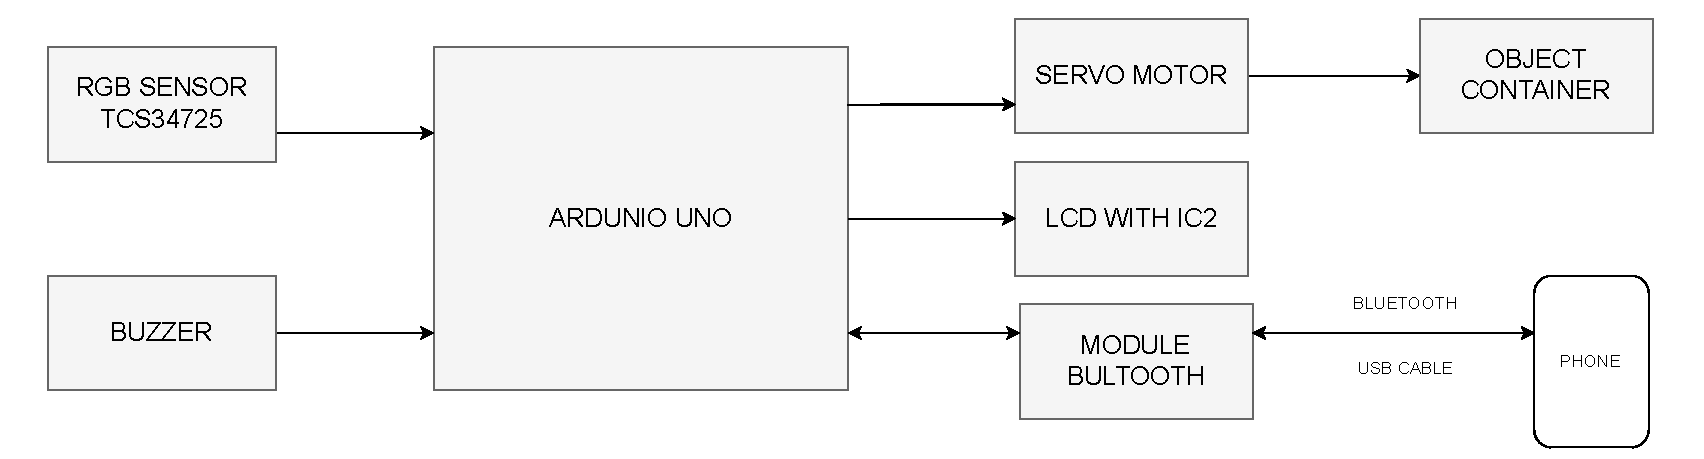
\includegraphics[width=1\textwidth]{IOT-Color-Based Object Sorting Machine/Block_Diagram.pdf}
    \captionof{figure}{Block diagram of the developed system.}
    \label{fig1}
    \end{center}
\vspace{1em}
\clearpage
\subsection{Components and Peripheral Devices}
The following are the main components used in the development of the Smart Water Pouring System:

\begin{itemize}
    \item \textbf{Arduino Uno Rev3:} The Arduino Uno Rev3 is a microcontroller board used for prototyping and controlling electronic projects, such as robotics, home automation, and sensor-based systems. It is based on the ATmega328P microcontroller and serves as a versatile platform for beginners and advanced users alike. The board supports digital and analog input/output, allowing it to interface with various components like sensors, motors, and displays. The Arduino Uno Rev3 typically has multiple pins, including: \textbf{VIN} connects to an external 7-12V power source or \textbf{5V} pin for a regulated 5V supply, \textbf{GND} connects to ground, \textbf{Digital I/O Pins} (14 pins, labeled 0-13, of which 6 support PWM) connect to components for input or output, and \textbf{Analog Input Pins} (6 pins, labeled A0-A5) connect to analog sensors. Additionally, it includes a \textbf{USB} port for programming and power (5V via USB) and a \textbf{Reset} pin/button to restart the board.
  \vspace{1em}
    \begin{center}
    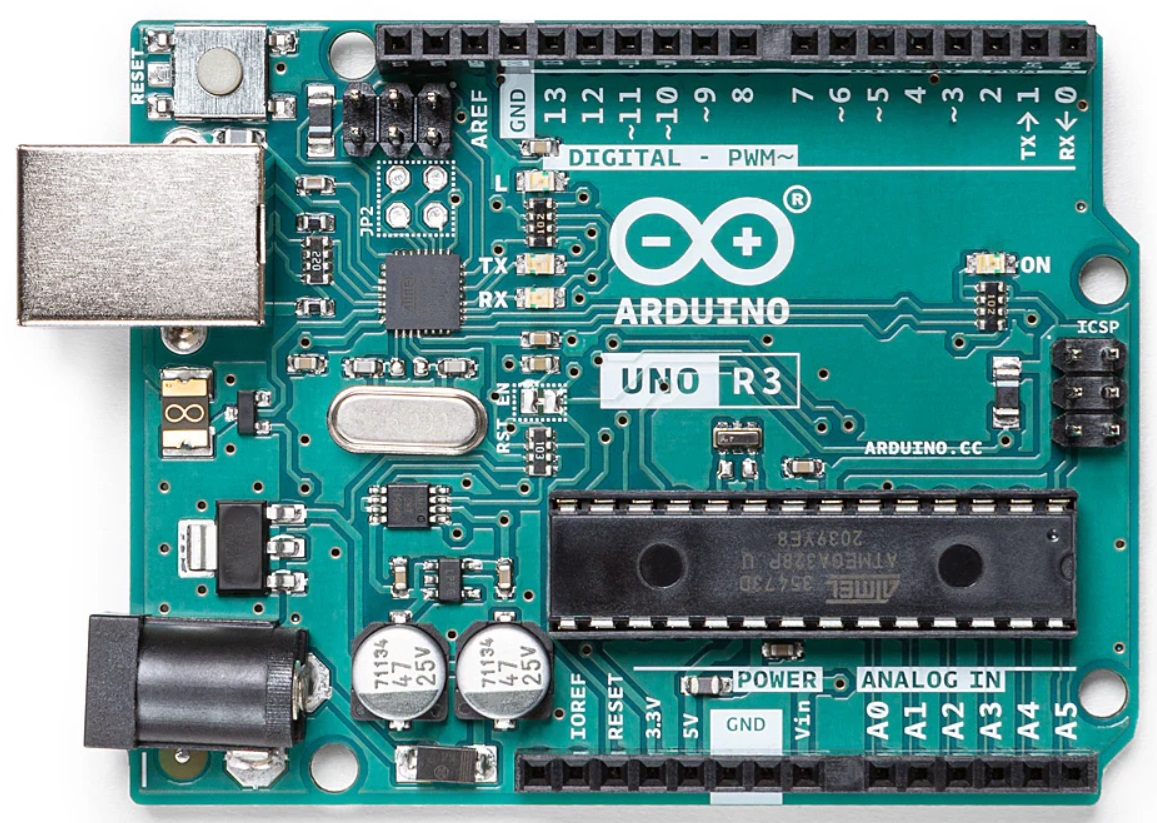
\includegraphics[width=0.4\textwidth]{IOT-Color-Based Object Sorting Machine/Arduino_Uno.jpg}
     \vspace{1em}
    \captionof{figure}{Arduino Uno Rev3.}
    \label{fig2}
    \end{center}

\vspace{6em}
    \item \textbf {TSC34725 Color Sensor:} The TCS34725 Color Sensor is used for detecting and measuring color (red, green, blue, and clear light) in electronic projects, such as color recognition, ambient light sensing, or display calibration, often interfaced with microcontrollers (e.g., Arduino or NodeMCU). It features an integrated IR-blocking filter and high-sensitivity photodiodes, providing accurate color and light intensity data via an I2C interface. The TCS34725 typically has six pins: \textbf{VCC} connects to a 3.3V or 5V power source, \textbf{GND} connects to ground, \textbf{SDA} is the serial data pin (connects to the SDA pin of the microcontroller), \textbf{SCL} is the serial clock pin (connects to the SCL pin of the microcontroller), \textbf{INT} (interrupt) signals when light levels exceed programmed thresholds, and \textbf{LED} controls an optional onboard LED for illumination (if present on the module). 

   
    \begin{center}
    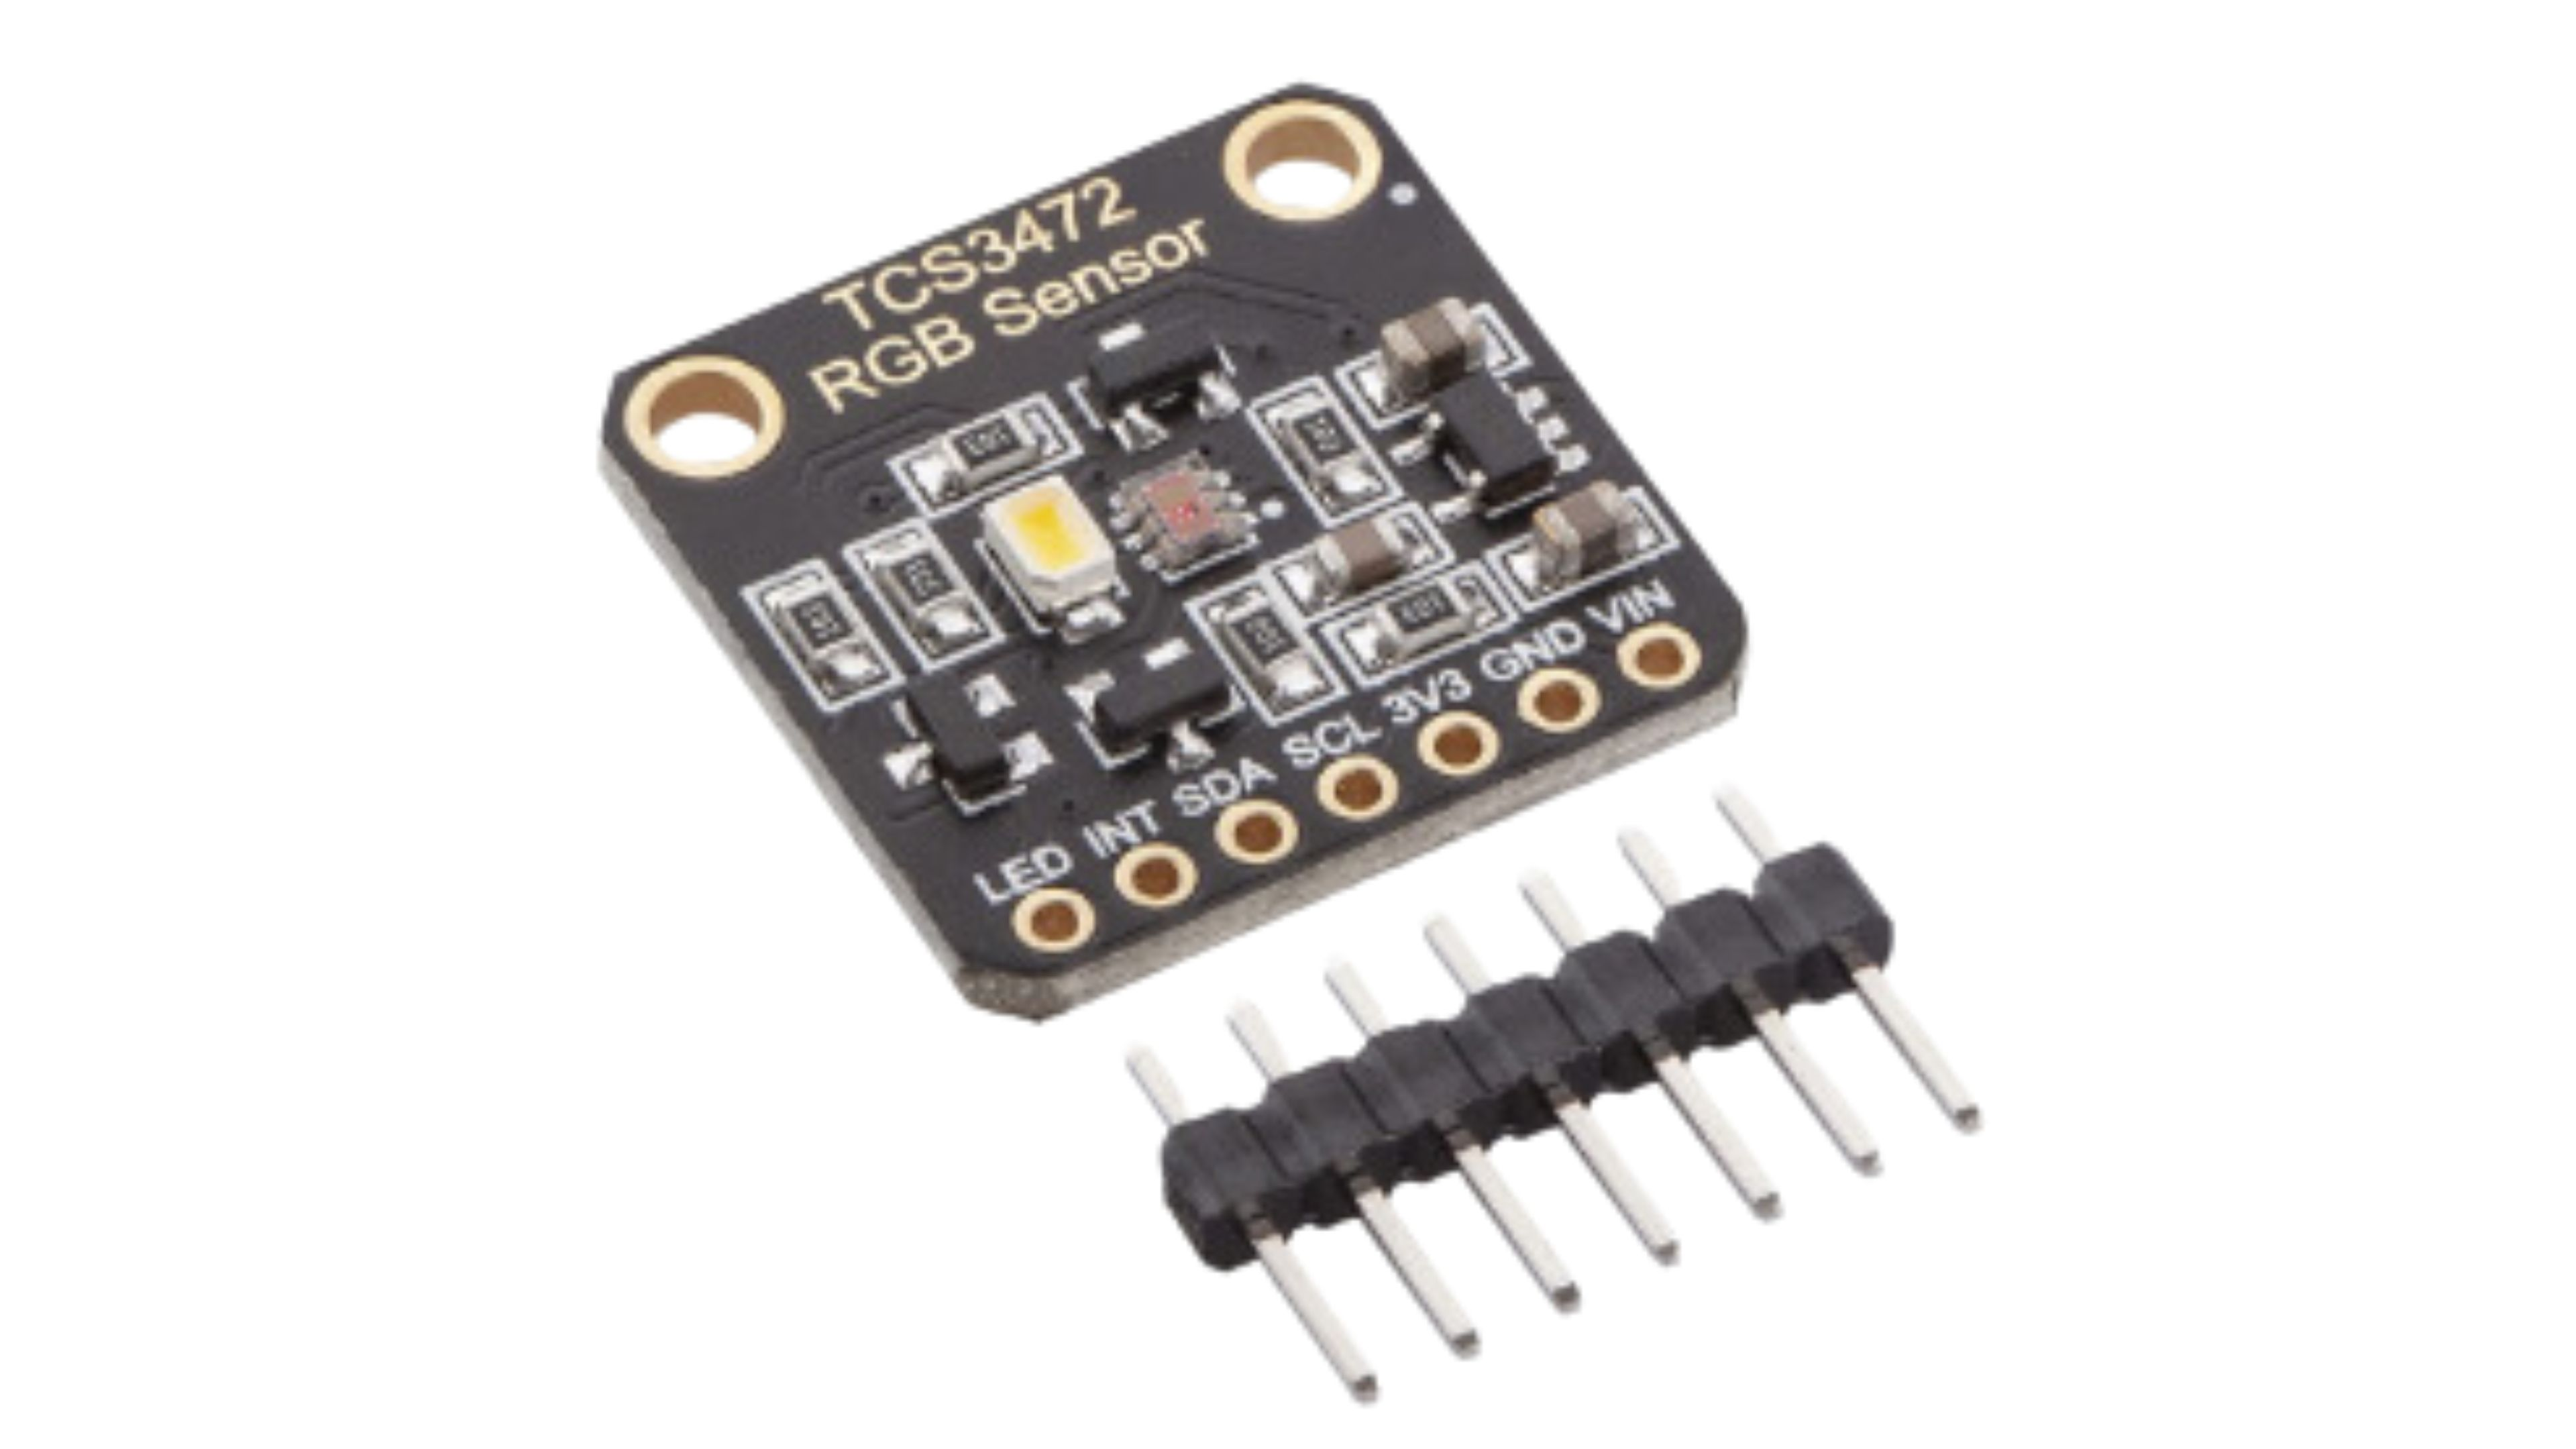
\includegraphics[width=0.6\textwidth]{IOT-Color-Based Object Sorting Machine/TSC34725_Color_Sensor.jpg}
    \captionof{figure}{TSC34725 Color Sensor.}
    \label{fig3}
    \end{center}
\vspace{6em}
    \item \textbf{Bluetooth Module (HC-05):} The HC-05 Bluetooth module is used for wireless communication between devices, such as connecting microcontrollers (e.g., Arduino or NodeMCU) to smartphones, PCs, or other Bluetooth-enabled devices. It supports both master and slave modes, allowing it to send and receive data wirelessly. The HC-05 module typically has six pins: \textbf{VCC} connects to a 3.3V or 5V power source, \textbf{GND} connects to ground, \textbf{TXD} is the transmit data pin (connects to the RX of the microcontroller), \textbf{RXD} is the receive data pin (connects to the TX of the microcontroller), \textbf{STATE} indicates the connection status (HIGH for connected), and \textbf{EN} enables or disables the module, used for configuration.

    \begin{center}
    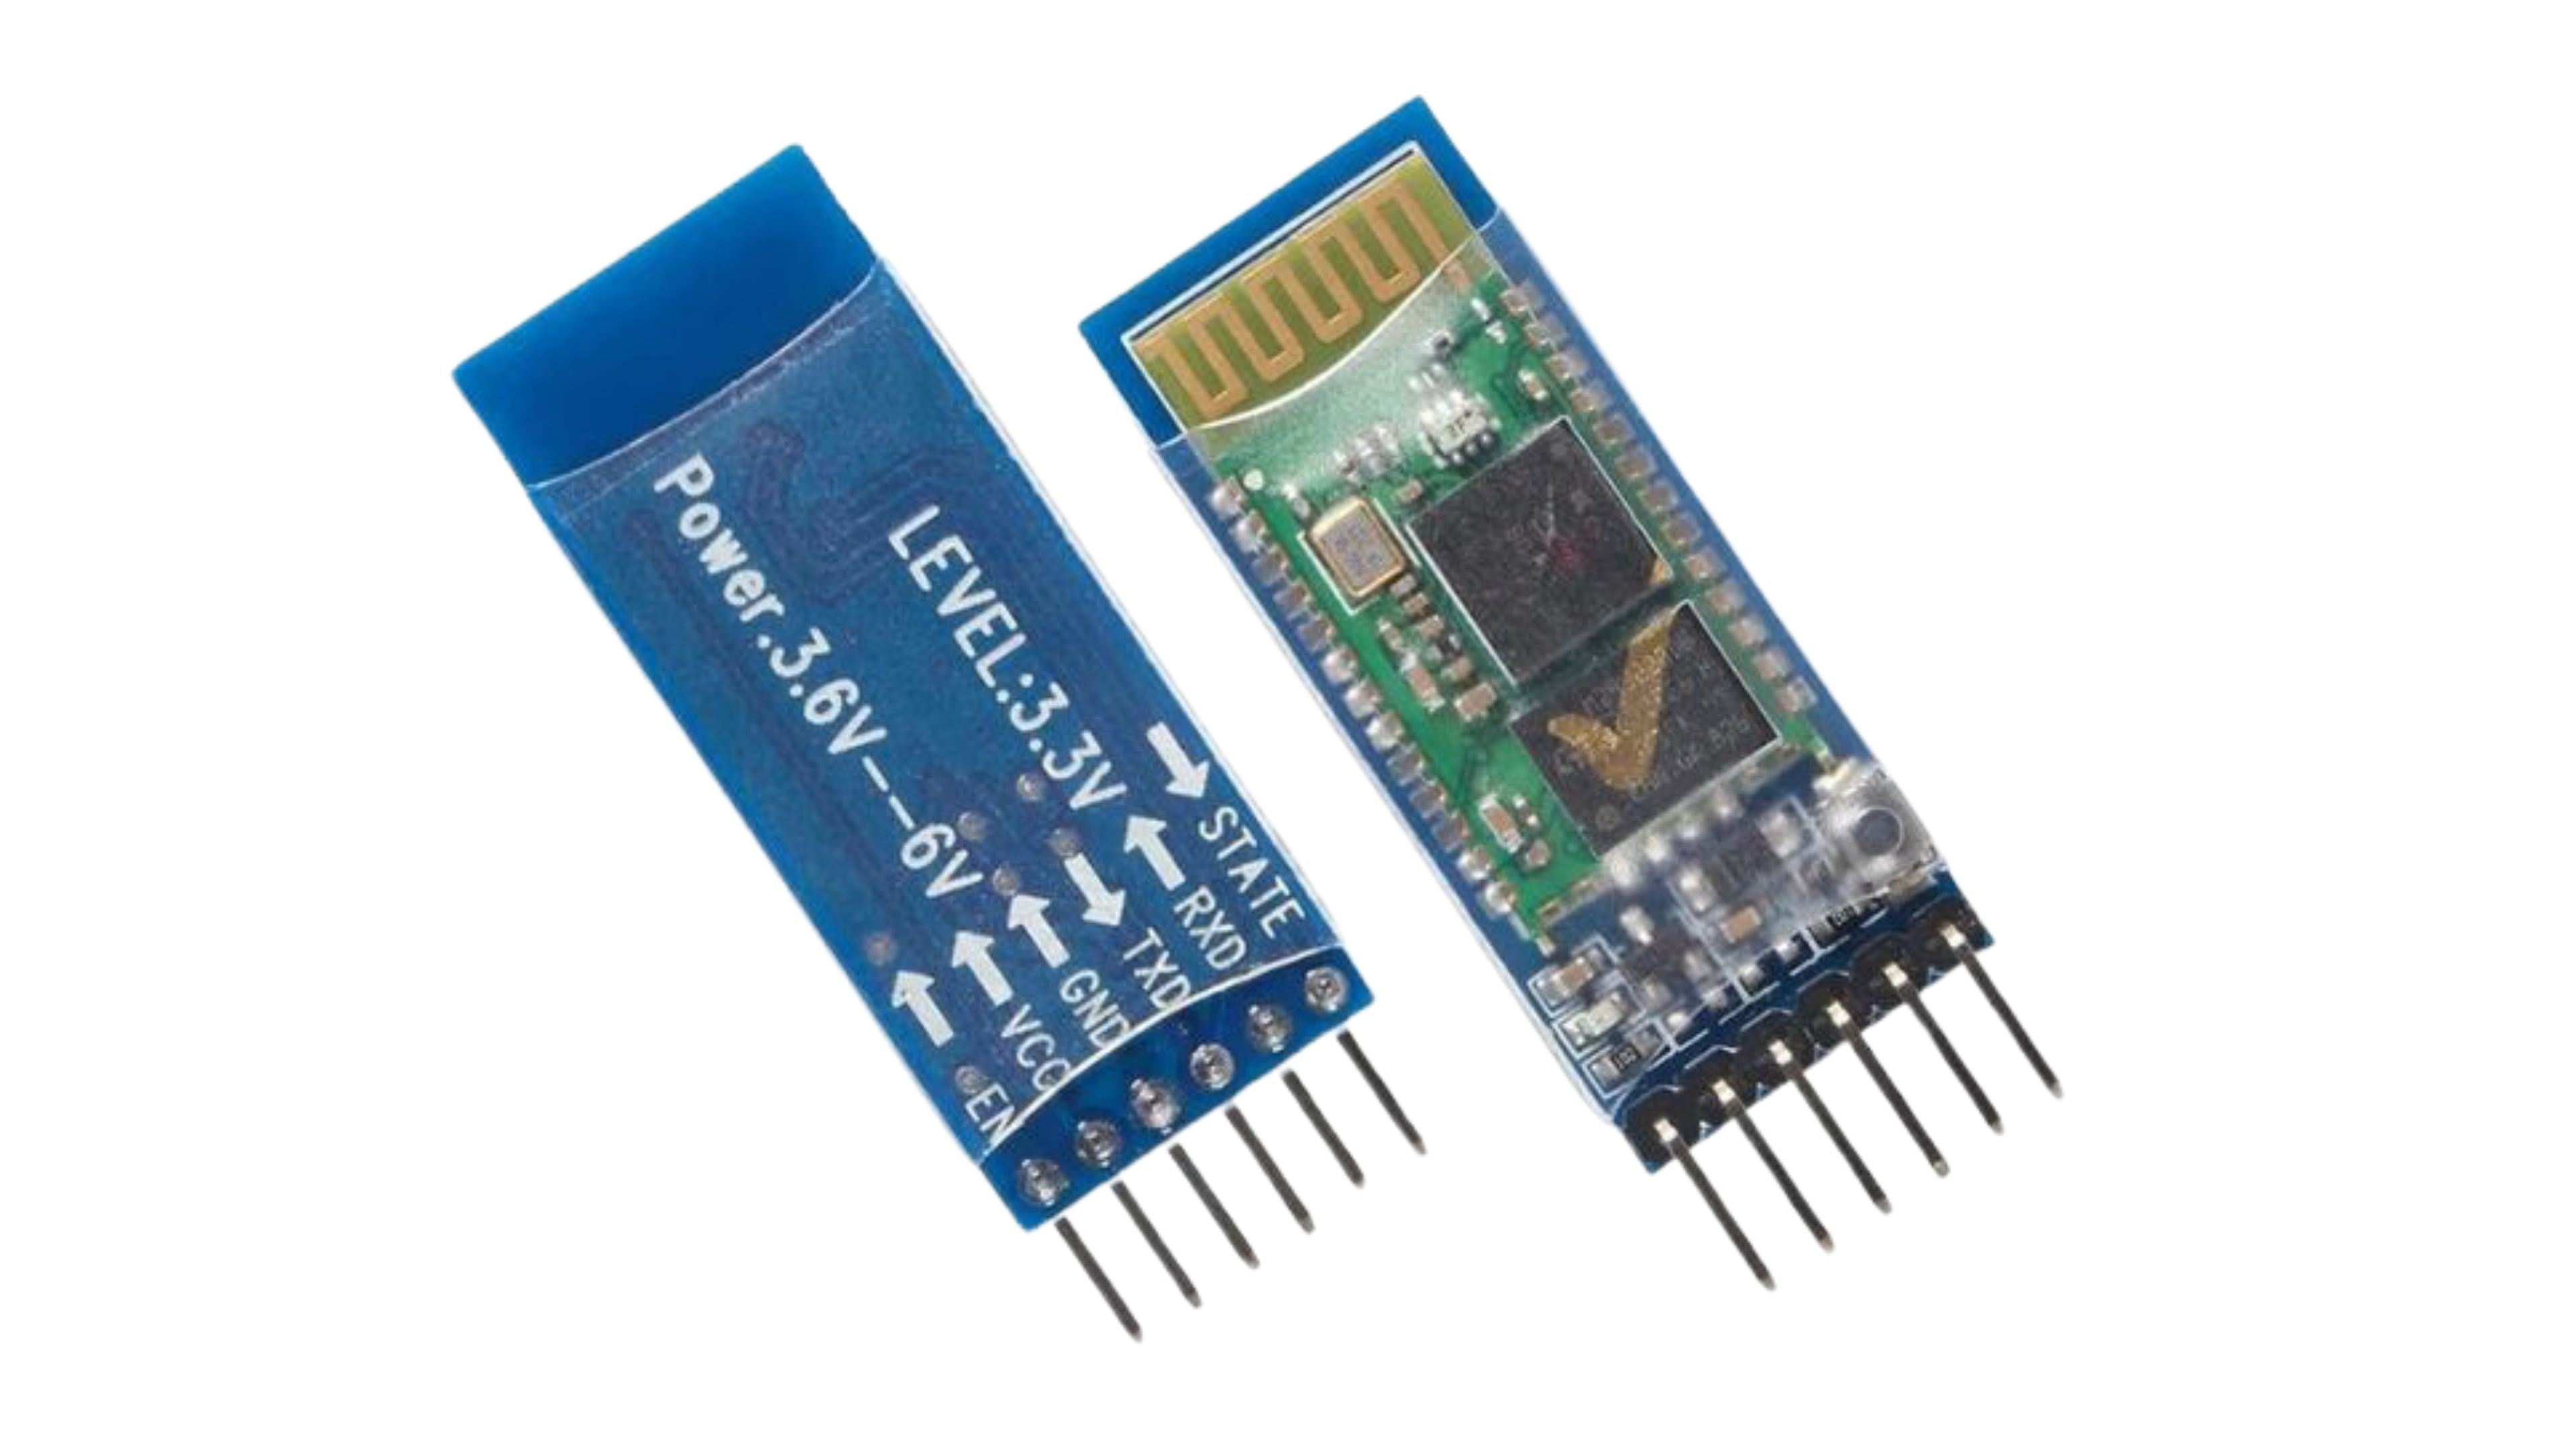
\includegraphics[width=0.6\textwidth]{IOT-Color-Based Object Sorting Machine/Bluetooth_Module_HC05.jpg} % Replace with actual image path
    \captionof{figure}{Bluetooth Module (HC-05).}
    \label{fig4}
    \end{center}
  
\vspace{8em}
    \item \textbf{Servo Motor:} The Servo Motor is used for precise control of angular position in various devices, such as robotics, remote-controlled vehicles, or automated systems. It is commonly interfaced with microcontrollers (e.g., Arduino or NodeMCU) to achieve accurate rotational movement. The servo motor typically operates in a closed-loop system with an internal feedback mechanism, allowing it to maintain a specified position. A standard hobby servo motor has three pins: \textbf{VCC} connects to a 4.8V to 6V power source (typically 5V), \textbf{GND} connects to ground, and \textbf{Signal} (or PWM) is the control pin (connects to a digital pin on the microcontroller), which receives pulse-width modulation (PWM) signals to determine the motor’s angle.

    \begin{center}
    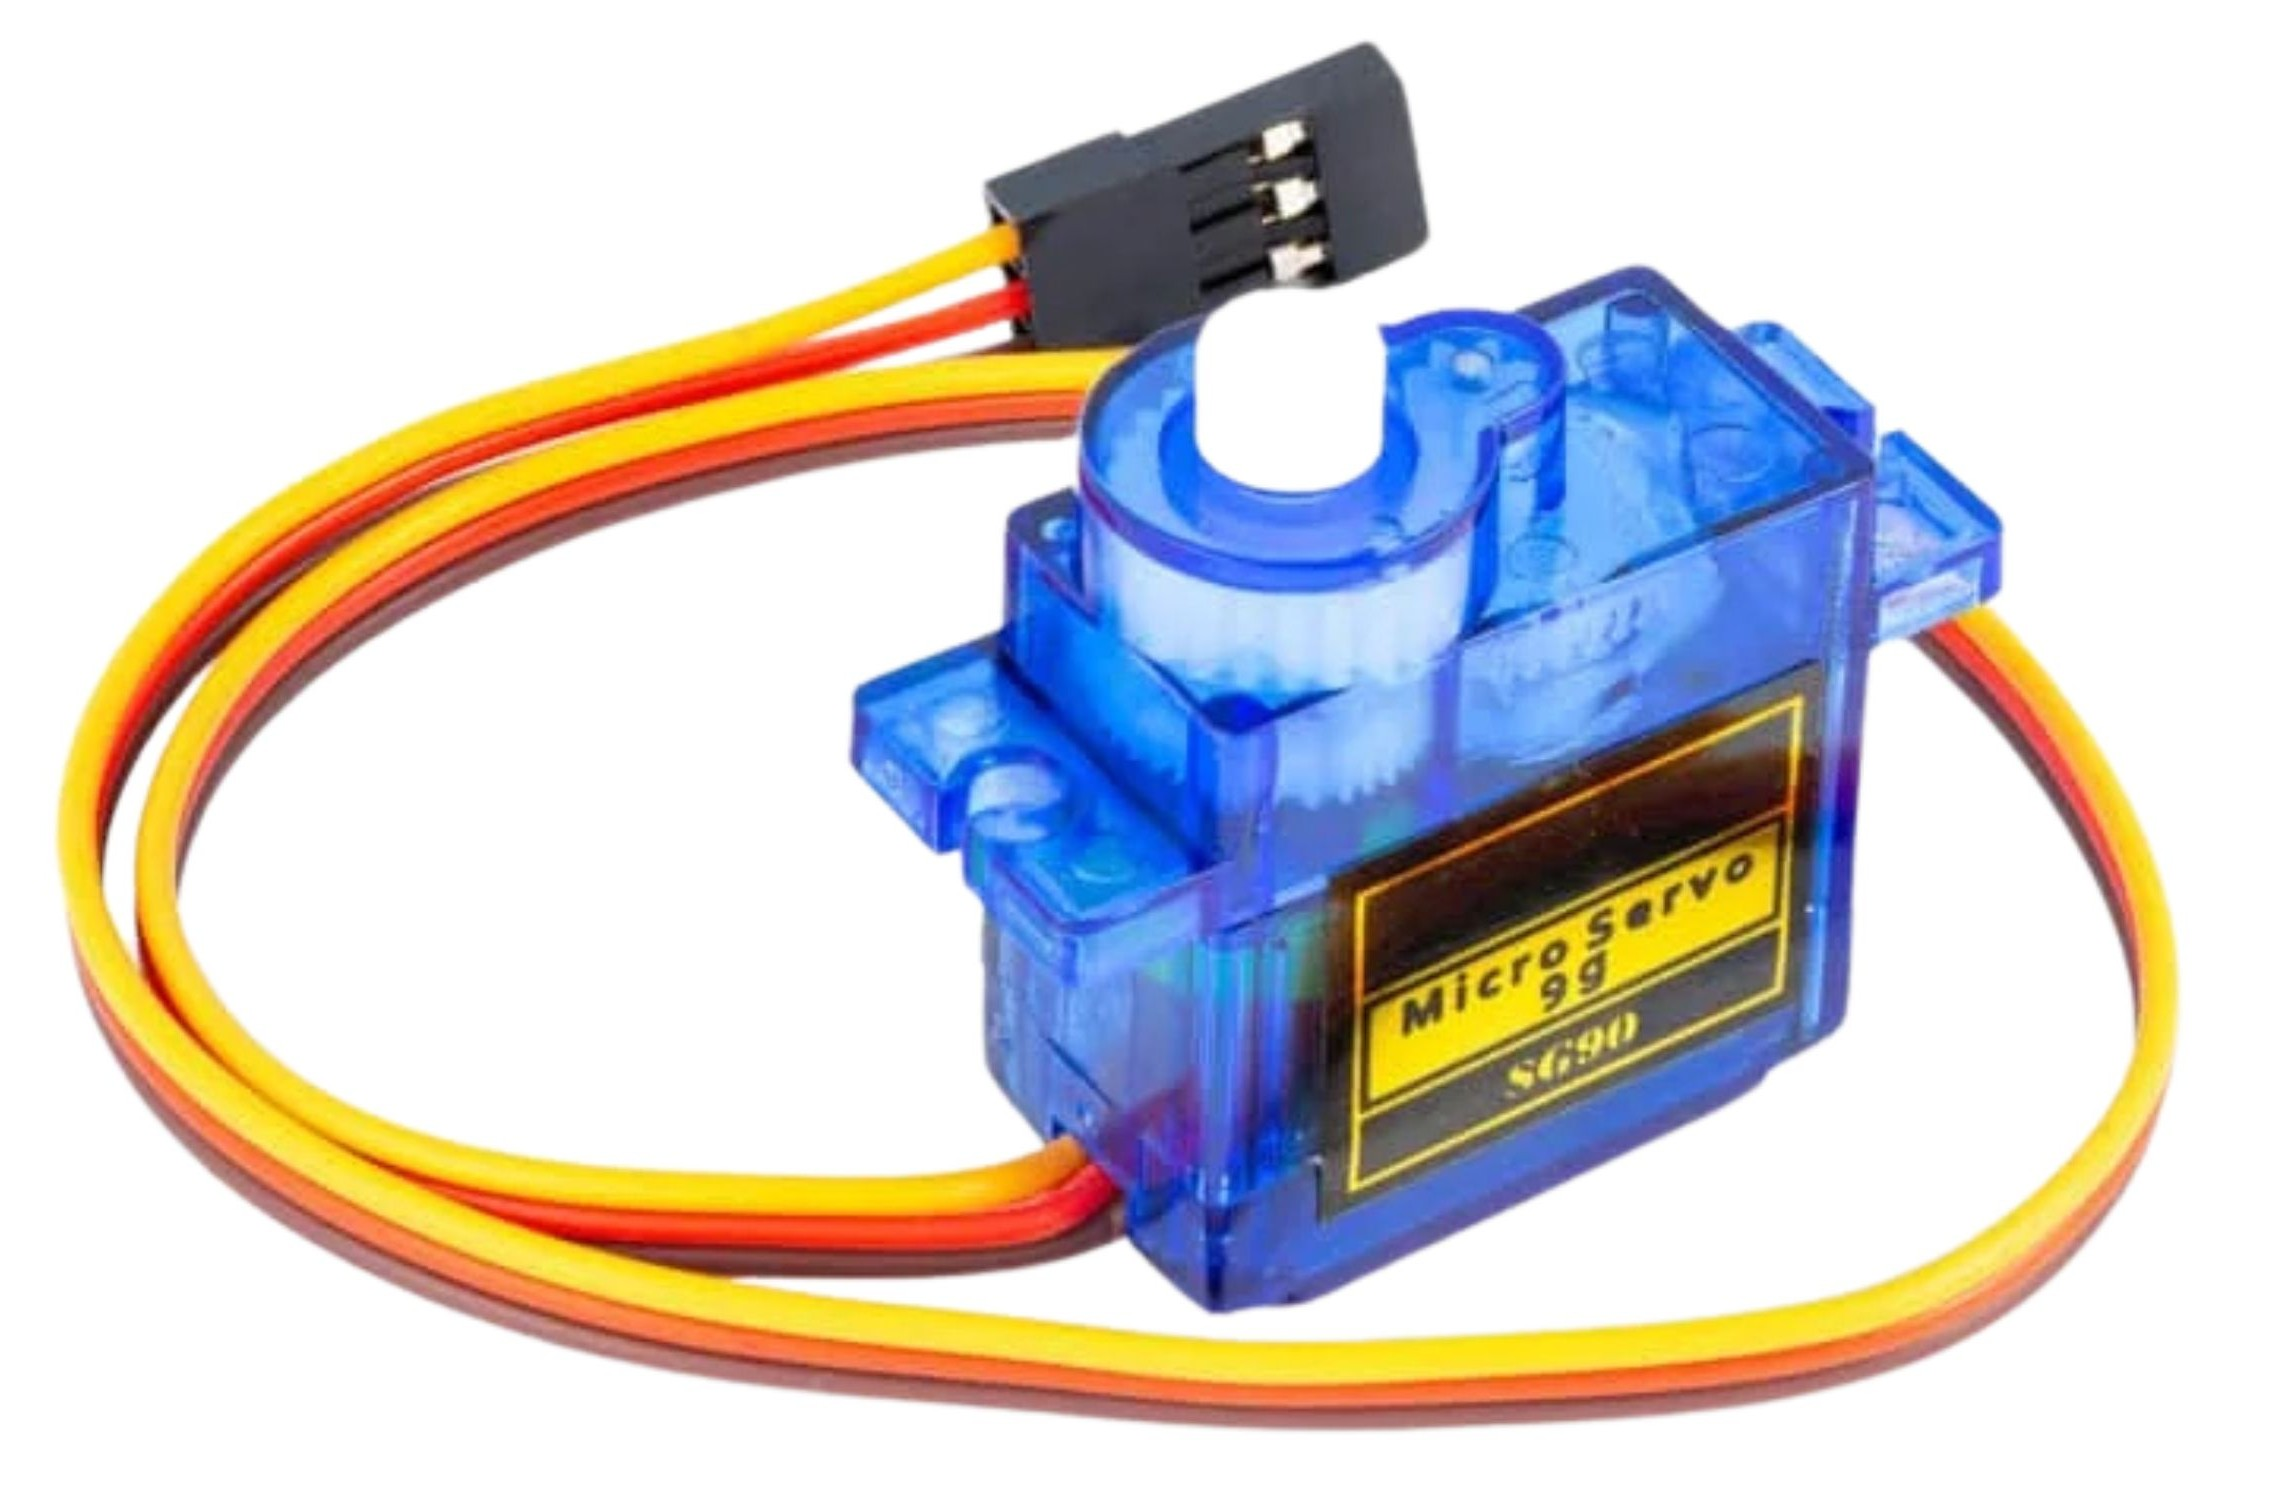
\includegraphics[width=0.45\textwidth]{IOT-Color-Based Object Sorting Machine/Servo_Moto.jpg} % Replace with actual image path
     \vspace{1em}
    \captionof{figure}{Servo Motor.}
    \label{fig5}
    \end{center}
\clearpage

    \item \textbf{LCD with I2C:} The LCD with I2C is used for displaying alphanumeric characters and simple graphics in electronic projects, such as showing sensor data or user interfaces on microcontrollers (e.g., Arduino or NodeMCU). It combines a standard liquid crystal display (LCD), typically 16x2 or 20x4 in size, with an I2C interface module, reducing the number of pins needed for communication. The I2C protocol enables efficient two-wire communication with a microcontroller. The LCD with I2C module typically has four pins: \textbf{VCC} connects to a 5V power source, \textbf{GND} connects to ground, \textbf{SDA} is the serial data pin (connects to the SDA pin of the microcontroller), and \textbf{SCL} is the serial clock pin (connects to the SCL pin of the microcontroller).

    \begin{center}
    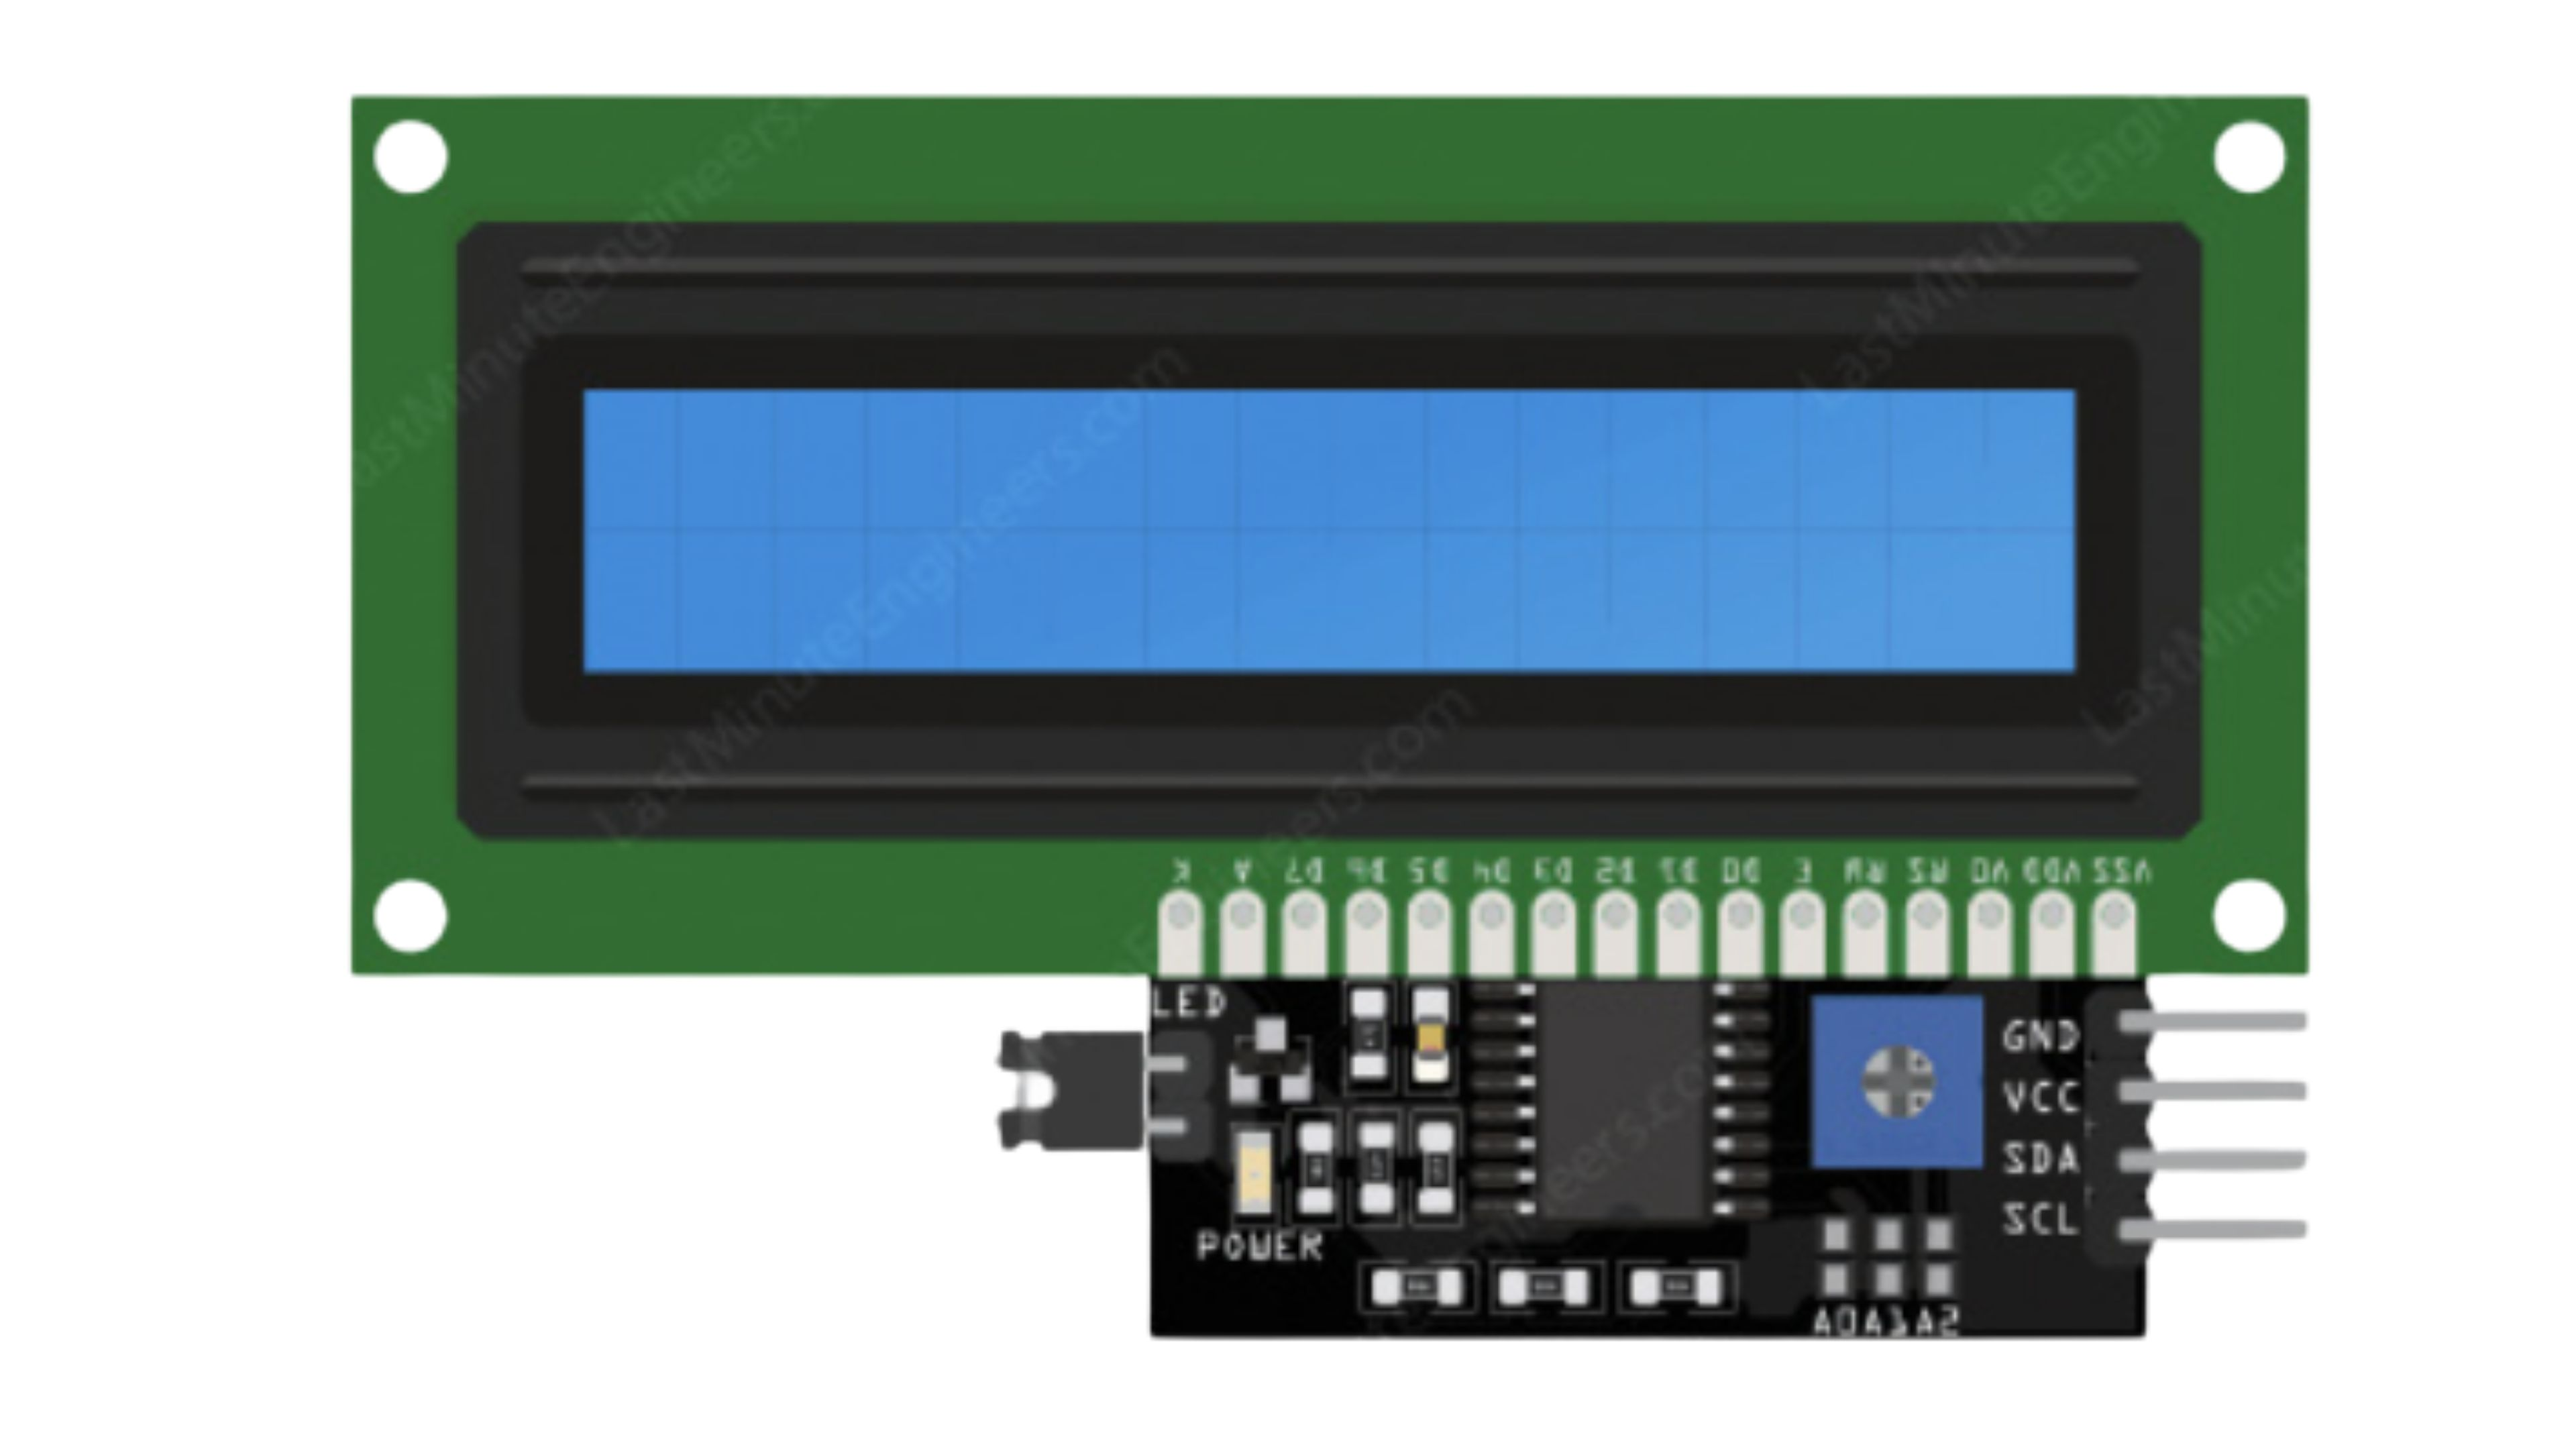
\includegraphics[width=0.525\textwidth]{IOT-Color-Based Object Sorting Machine/LCD_with_I2C.jpg} % Replace with actual image path
    \captionof{figure}{LCD with I2C.}
    \label{fig6}
    \end{center}

\vspace{6em}

    \item \textbf{Buzzer:} The Buzzer is used for generating audible signals or alerts in electronic projects, such as indicating events, alarms, or user feedback in systems controlled by microcontrollers (e.g., Arduino or NodeMCU). It can produce tones of varying frequencies depending on the input signal. Buzzers come in two main types: active buzzers (which generate sound with a fixed frequency when powered) and passive buzzers (which require an oscillating signal to produce sound). A typical buzzer has two pins: \textbf{VCC} connects to a 3.3V or 5V power source (depending on the buzzer type), and \textbf{GND} connects to ground. For passive buzzers, the VCC pin is often labeled as the signal pin and connects to a digital pin on the microcontroller to receive pulse-width modulation (PWM) or square wave signals for producing different tones.

    \begin{center}
    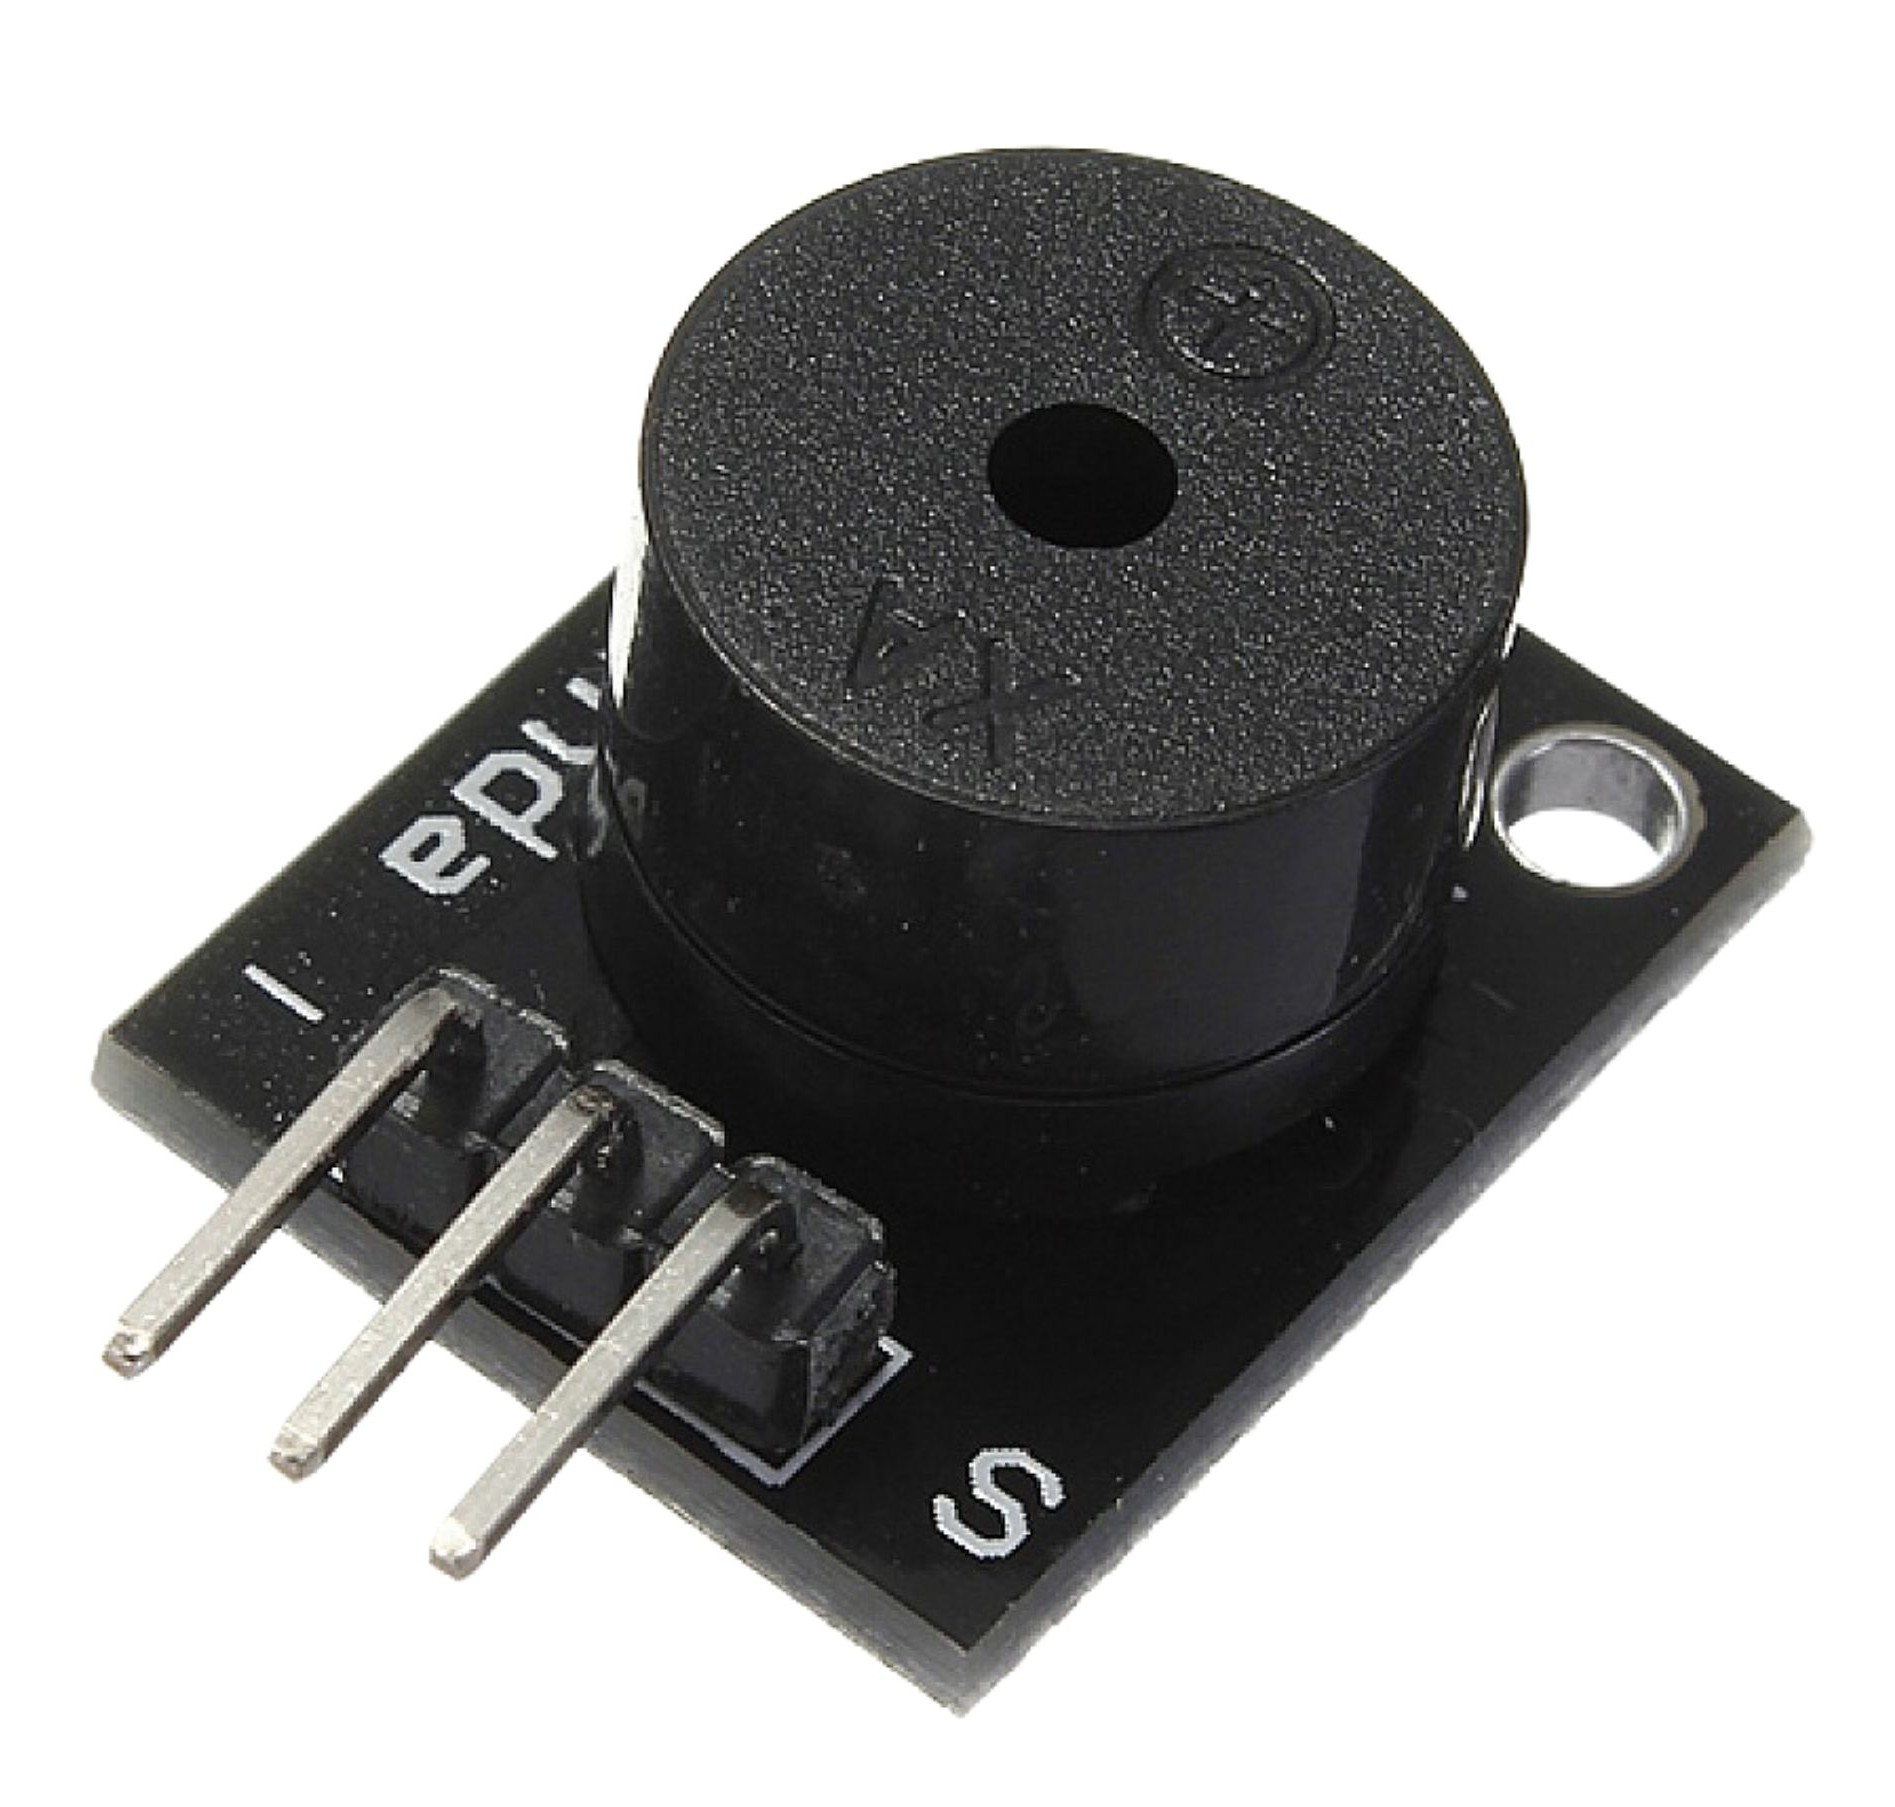
\includegraphics[width=0.35\textwidth]{IOT-Color-Based Object Sorting Machine/Buzzer.jpg} % Replace with actual image path
    \captionof{figure}{Buzzer.}
    \label{fig7}
    \end{center}
\end{itemize}
\clearpage

\vspace{2em}

Figure \ref{fig8} shows the schematic of the circuit interfacing for the developed Color-Based Object Sorting Machine, where the key components are connected to the Arduino Uno as follows:
    \begin{center}
    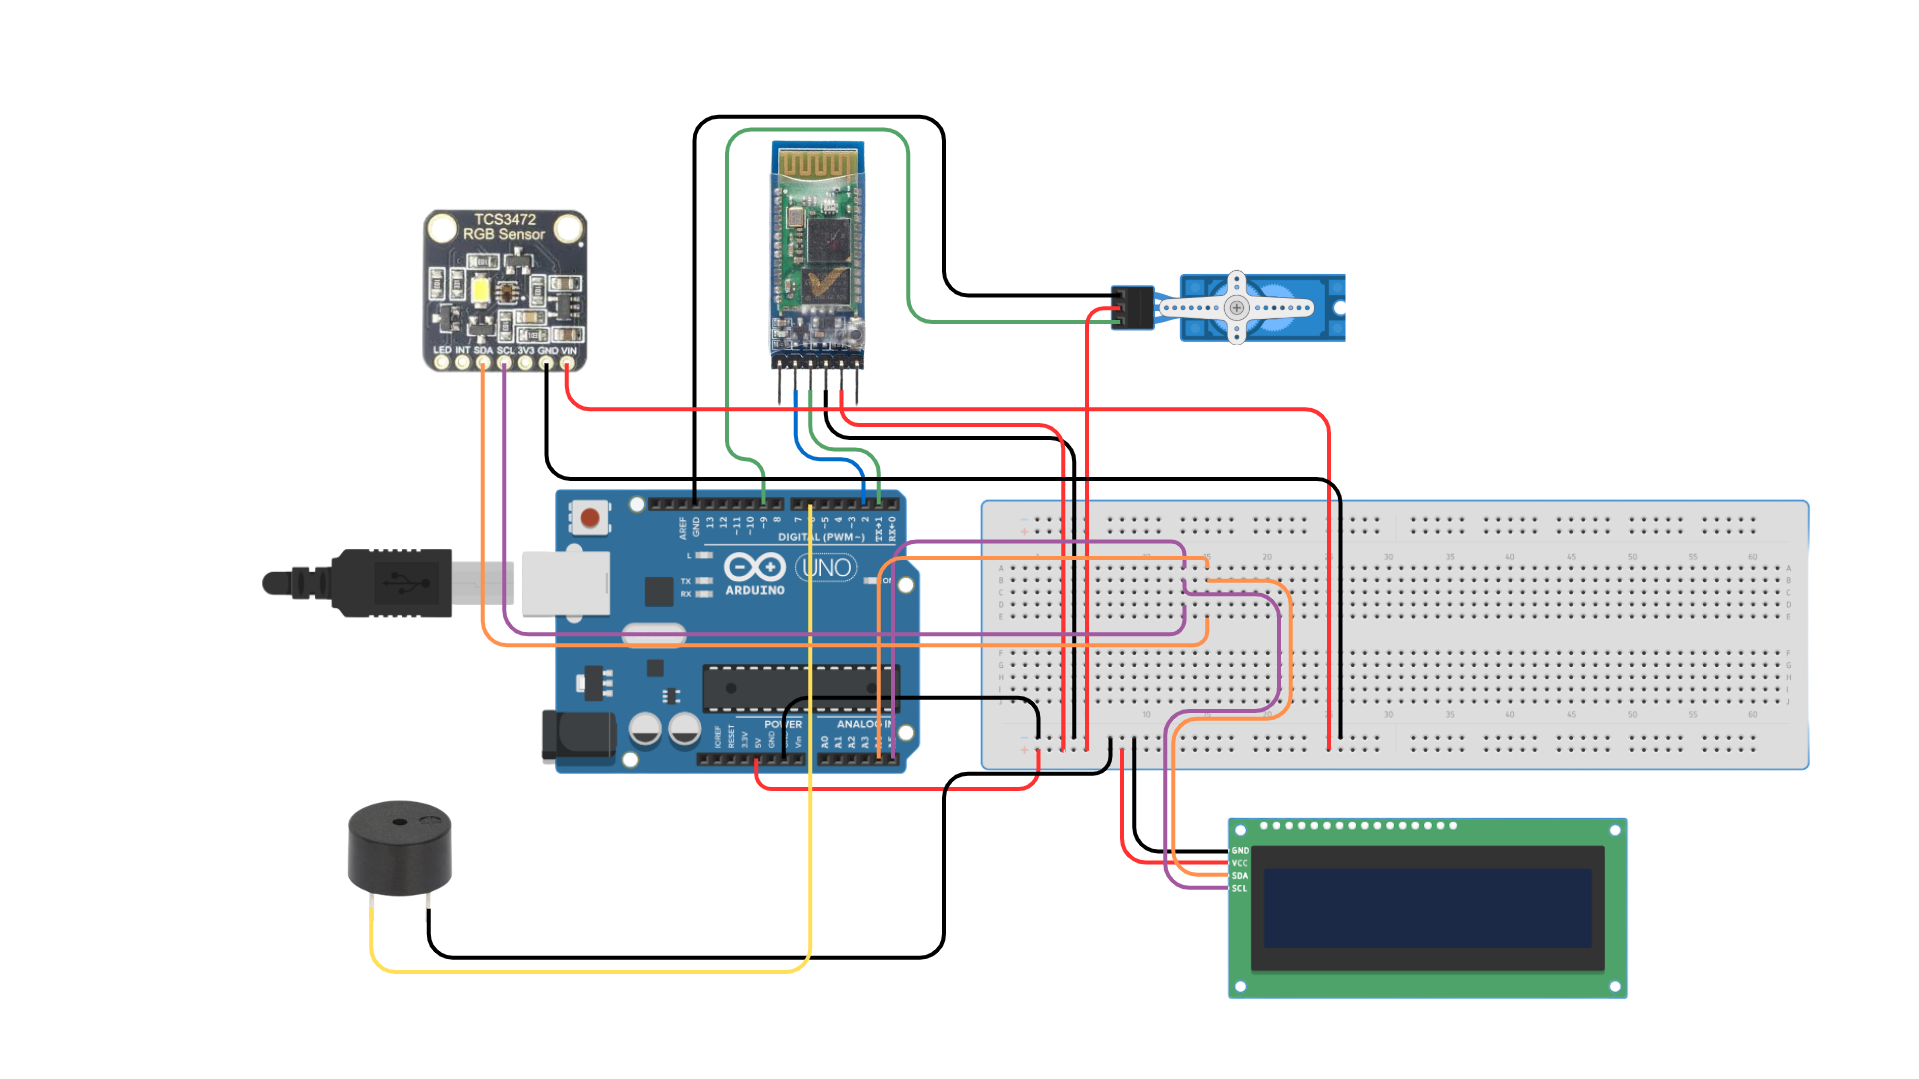
\includegraphics[width=\textwidth]{IOT-Color-Based Object Sorting Machine/Devices_and_Connection_Diagram.png}
    \captionof{figure}{Devices and Connection Diagram}
    \label{fig8}
    \end{center}
The system is connected as follows: Arduino Uno acts as the central processing unit, controlling the entire system. The Bluetooth module (HC-05) is connected with VCC to 5V, GND to GND, TXD to Pin 3 (with a voltage divider to reduce 5V to 3.3V), and RXD to Pin 2 on the Arduino, using SoftwareSerial for communication. The TCS34725 color sensor has VIN connected to 3.3V (or 5V, if supported—check datasheet), GND to GND, SDA to A4, and SCL to A5 for I2C communication. The I2C LCD screen is also connected using the I2C standard, with VCC to 5V, GND to GND, SDA to A4, and SCL to A5.
The system also includes a buzzer, with one pin connected to Pin 6 on the Arduino and the other pin to GND, allowing it to emit alert sounds. The servo motor has VCC connected to an external 5V power supply (with GND common to Arduino), GND to GND, and the control signal connected to Pin 9 on the Arduino.
This system is capable of wireless communication via Bluetooth, color detection using the TCS34725 sensor, displaying information on the LCD screen, emitting alert sounds with the buzzer, and controlling the servo motor based on collected data. With these functionalities, the system can be applied in color recognition, object-sorting robots, or other IoT applications.
 \vspace{3em}
\begin{table}[htb]
    \caption{Interfacing between Arduino Uno and Its Components for Color-Based Object Sorting Machine}
    \label{tab:interfacing-components}
    \centering
    \begin{tabular}{|l|l|l|l|l|l|}
        \hline
        \textbf{Arduino Uno Pin} & \textbf{TCS34725 Color Sensor} & \textbf{LCD Display (I2C)} & \textbf{Servo Motor} & \textbf{Bluetooth Module (HC-05/HC-06)} & \textbf{Buzzer} \\ \hline
        \textbf{GND}         & GND                   & GND         & GND        & GND            & GND            \\ \hline
        \textbf{3.3V/5V (VCC)} & VIN                   & VCC         & --          & --             & --             \\ \hline
        \textbf{5V (VCC)}    & --                    & --          & VCC         & VCC            & VCC            \\ \hline
        \textbf{D2 (RX)}     & --                    & --          & --          & RXD (Receive)  & --             \\ \hline
        \textbf{D3 (TX)}     & --                    & --          & --          & TXD (Transmit) & --             \\ \hline
        \textbf{A4 (SDA)}    & SDA                   & SDA         & --          & --             & --             \\ \hline
        \textbf{A5 (SCL)}    & SCL                   & SCL         & --          & --             & --             \\ \hline
        \textbf{D6}          & --                    & --          & --          & --             & IN (Control)   \\ \hline
        \textbf{D9}          & --                    & --          & Signal (Control) & --             & --             \\ \hline
    \end{tabular}
\end{table}
\clearpage

\subsection{Software Programming}


To enhance the functionality and usability of the Color-Based Object Sorting Machine, a custom mobile app is developed using MIT App Inventor. This app facilitates Bluetooth communication with the system, allowing users to control the sorting process remotely. The following steps outline the creation process:
 \vspace{3em}
\paragraph{Step 1: Access MIT App Inventor}  
Begin by accessing the MIT App Inventor platform, a user-friendly tool for creating mobile applications. Navigate to https://appinventor.mit.edu using a web browser, click on the "Create Apps" button, and log in with your Google account credentials. Once logged in, you will be directed to the main interface, which provides options for designing and programming your app. This step sets the foundation for app development.

\begin{center}
    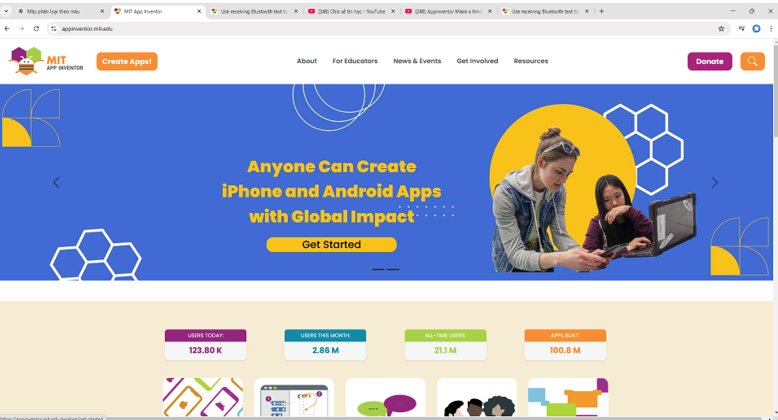
\includegraphics[width=0.9\linewidth]{Access MIT App Inventor.png}
    \captionof{figure}{Access MIT App Inventor}
    \label{fig1}
    \end{center}
 \vspace{3em}
\noindent


\paragraph{Step 2: Create a New Project}  
Start by creating a new project to build the Bluetooth app. In the top menu, click on "Projects", select the "Start new project" option, and a dialog box will appear. Enter a name for your project, such as ColorSorterApp, to identify it clearly among other projects. After naming, press OK to initialize the project, which will create a blank canvas where you can design and program your app.

\begin{center}
    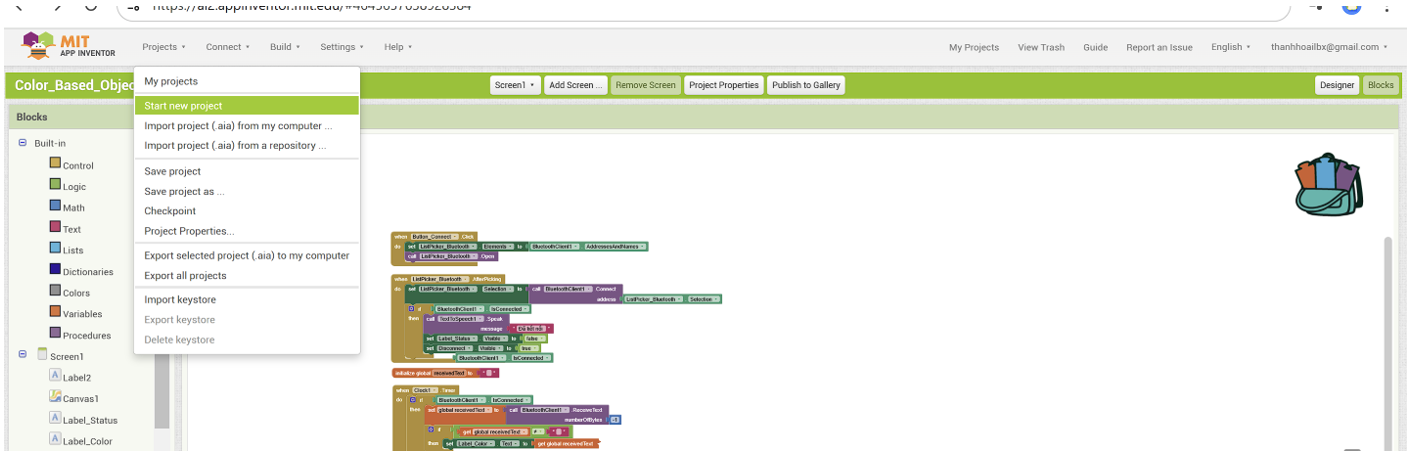
\includegraphics[width=0.9\linewidth]{IOT Create a new Project.png}
    \captionof{figure}{Create new project}
    \label{fig1}
    \end{center}
\noindent

\begin{center}
    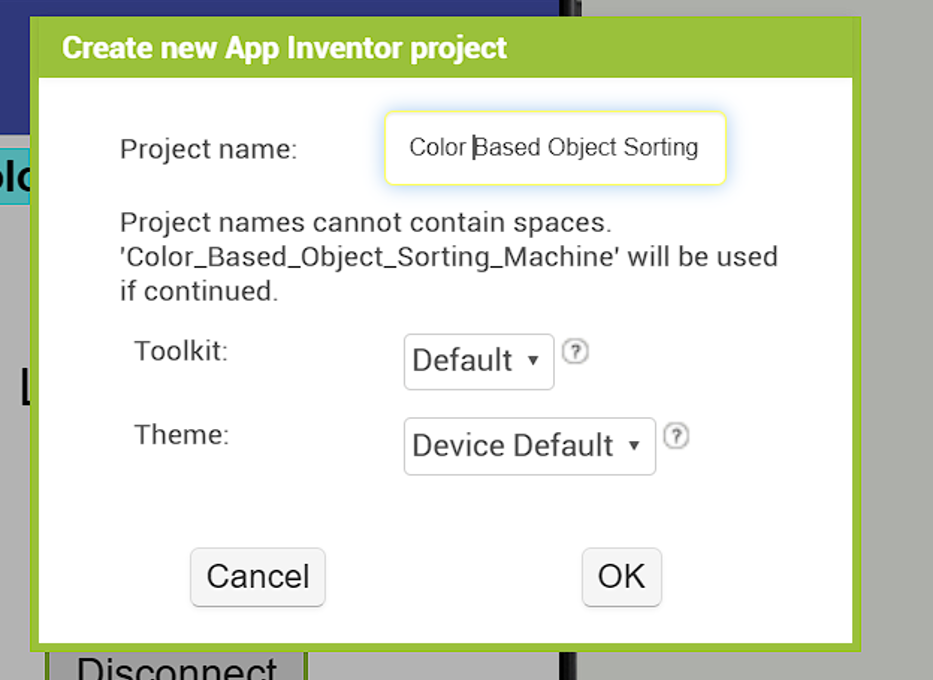
\includegraphics[height=10cm, width=0.9 \textwidth]{IOT Create a new Project1.png}
    \captionof{figure}{Enter a name for your project}
    \label{fig1}
    \end{center}
     \vspace{1em}
\noindent
\clearpage

\paragraph{Step 3: Design the User Interface}  
Begin by creating an intuitive and user-friendly interface using components from the Palette section. Drag a Button into the Viewer and rename it to "Pair with Bluetooth", allowing users to connect to the sorting machine. Below this button, add a Label to display the connection status, such as "Status: Disconnected". Customize the text properties—such as font size, color, and alignment—using the Properties panel for better visibility. You may also add extra buttons to start and stop the sorting process or display real-time status updates.

\begin{center}
    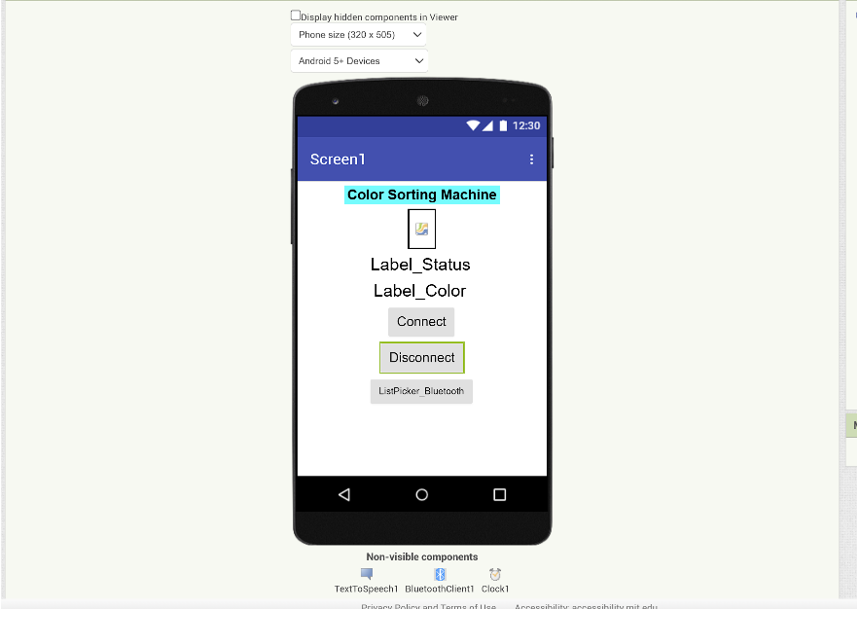
\includegraphics[height=10cm, width=0.9\textwidth]{IOT Design the User Interface.png}
    \captionof{figure}{Design the User Interface}
    \label{fig1}
    \end{center}
    \vspace{3em}
\noindent


\paragraph{Step 4: Integrate Bluetooth Functionality}  
To establish communication between the app and the sorting machine, add a Bluetooth Client component. Navigate to the Connectivity section in the Palette, then drag the Bluetooth Client into the Non-visible Components area. This component enables seamless data exchange with the Bluetooth module of the sorting machine. Ensure that it is correctly configured for stable connections and efficient communication.

% \begin{center}
%     \includegraphics[width=0.4\linewidth]{4.jpg}
%     \captionof{figure}{Add Bluetooth Client Component}
%     \label{fig1}
%     \end{center}
% \noindent
\begin{center} 
    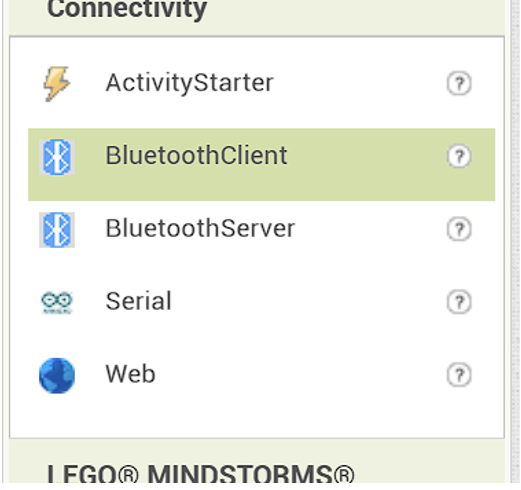
\includegraphics[width=0.4\linewidth]{The Non-visible Components area.png}
    \captionof{figure}{Integrate Bluetooth Functionality}
    \label{fig1}
    \end{center}
    \vspace{3em}
\noindent

\paragraph{Step 5: Implement Logic with Blocks}  
Switch to the Blocks tab to define how the app behaves. Use logic blocks to program the "Pair with Bluetooth" button so that it scans for available Bluetooth devices, lists them, and allows the user to select and connect to the sorting machine. Implement blocks for data transmission, ensuring that the app can send sorting commands and receive status updates, such as detected object colors or errors. Update the status label dynamically based on the connection state and received data.

\begin{center}
    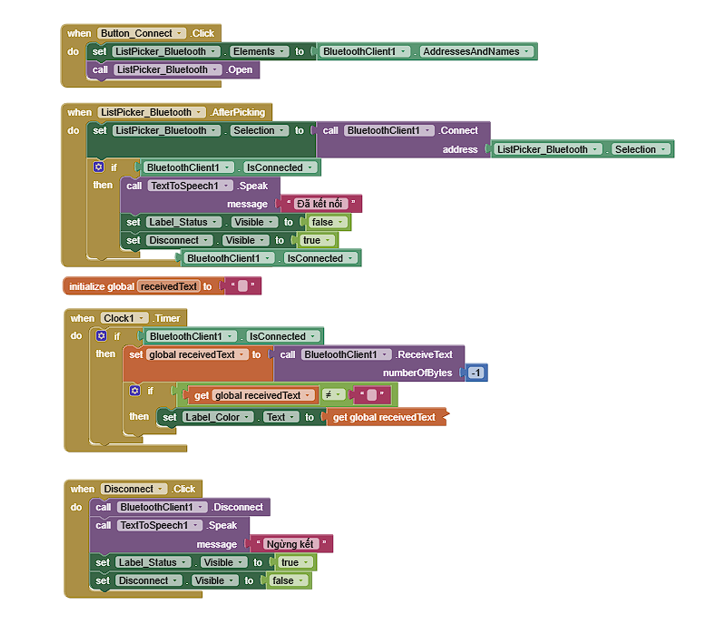
\includegraphics[width=0.9\textwidth]{Program the App with Blocks.png}
    \captionof{figure}{Implement Logic with Blocks}
    \label{fig1}
    \end{center}
      \vspace{3em}
\noindent 

\paragraph{Step 6: Test the App} 
Before finalizing the app, test its performance using the MIT AI2 Companion app. Open the companion app on a mobile device, then in MIT App Inventor, navigate to Connect > AI Companion to generate a QR code. Scan this QR code to instantly load and test the app in real time. Check if the Bluetooth pairing, sorting commands, and status updates work correctly. Make any necessary adjustments to ensure smooth operation.
\begin{center}
    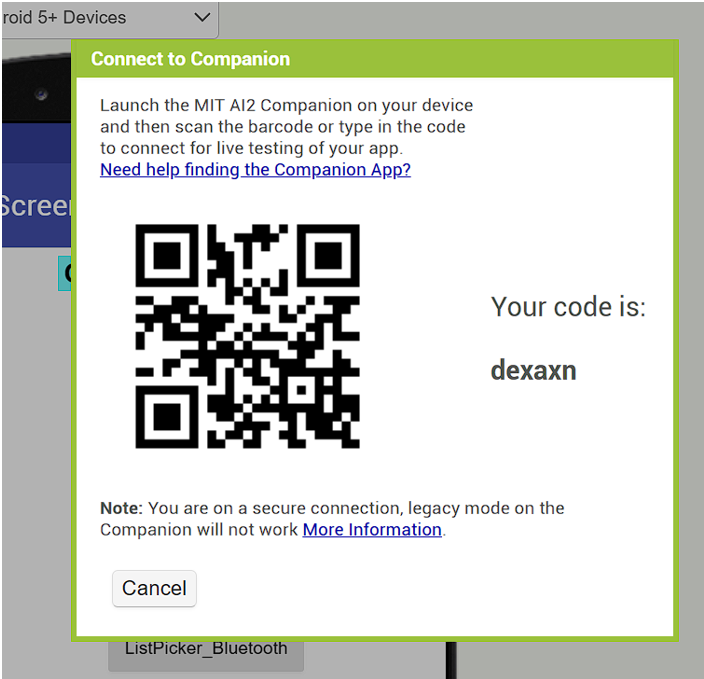
\includegraphics[height=10cm, width=0.7\linewidth]{QR Code.png}
    \captionof{figure}{QR code}
    \label{fig1}
    \end{center}
      \vspace{3em}
\noindent


\paragraph{Step 7: Save and Export the Project}  
Once the app functions as expected, save and export it for future use or sharing. Click on "Projects" in the top menu and select "Export selected project (.aia)..." to download the project file. This file allows you to re-import the app later for modifications. Additionally, you can generate an APK file to install the app on other devices, making it accessible for use with multiple sorting machines.

\begin{center}
    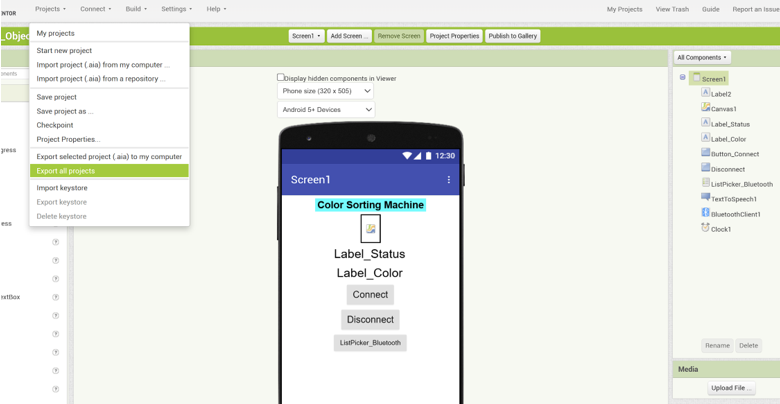
\includegraphics[width=0.9\textwidth]{Export selected project.png}
    \captionof{figure}{Export selected project}
    \label{fig1}
    \end{center}
      \vspace{3em}
\noindent
\clearpage

\subsection{Programming Flowchart}
\begin{center}
    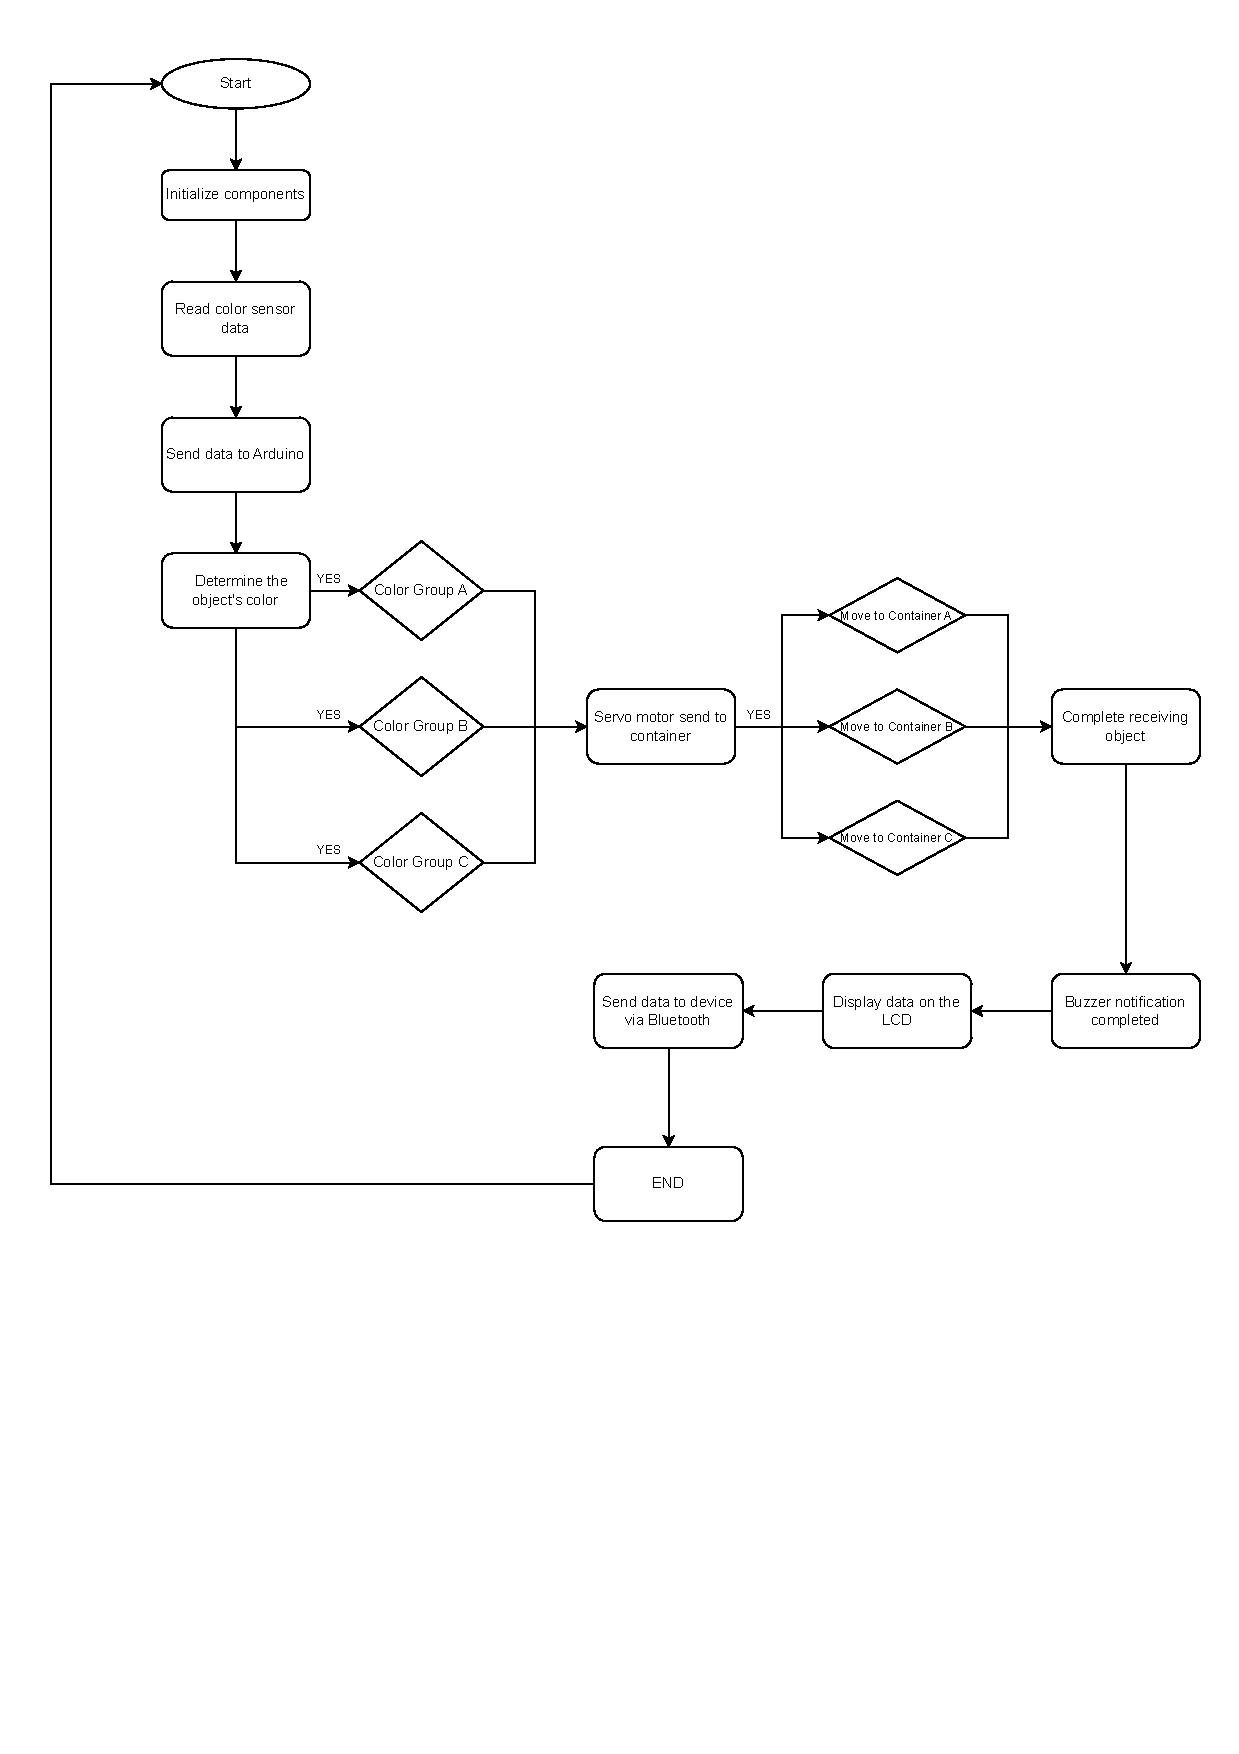
\includegraphics[width=1\textwidth, trim=0 7cm 0 0, clip]{IOT-Color-Based Object Sorting Machine/Flow_Chart.pdf}
    \captionof{figure}{Flowchart of Color-Based Object Sorting Machine}
    \label{fig1}
\end{center}
\noindent

\textbf{Step 1: Initialize Components}  
The system begins by initializing all hardware and software components to ensure seamless functionality. This involves configuring the Arduino to set up serial communication, initializing the color sensor for detecting object colors, setting up the servo motor for sorting, and preparing the LCD for displaying real-time data. Input pins for the sensors and actuators are also defined at this stage. By ensuring all components are correctly initialized, the system is ready to process and sort objects efficiently.

\vspace{0.5cm}
\noindent

\textbf{Step 2: Read Color Sensor Data}  
The color sensor continuously scans objects placed in the detection area and captures their color data. This information is crucial for categorizing the object into predefined groups. The sensor detects variations in red, green, and blue values, which help in determining the object's color.

\vspace{0.5cm}
\noindent

\textbf{Step 3: Send Data to Arduino}  
Once the color sensor captures the object’s color, the data is sent to the Arduino for processing. The Arduino receives the color information and analyzes it to determine the appropriate category for the object. Based on predefined thresholds, the system classifies the object into one of the color groups.

\vspace{0.5cm}
\noindent


\textbf{Step 4: Determine the Object's Color}  
The system compares the received color data against predefined color groups including Color Group A, Color Group B, and Color Group C. If the detected color matches one of these groups, the system proceeds with sorting.

\vspace{0.5cm}
\noindent


\textbf{Step 5:Activate Servo Motor for Sorting}  
After determining the object's color, the Arduino sends a signal to the servo motor to move the object towards the correct container. The motor positions itself based on the predefined sorting algorithm to ensure precise placement of the object.

\vspace{0.5cm}
\noindent

\textbf{Step 6: Move Object to the Correct Container}  
The servo motor directs the object to its respective container. It moves to Container A for Color Group A, Container B for Color Group B, and Container C for Color Group C. Once the object reaches the designated container, the sorting process is considered successful.
\vspace{0.5cm}
\noindent

\textbf{Step 7: Complete Receiving Object}
After the object is placed in the correct container, the system registers the completion of the sorting process. This step ensures that each object is accounted for and placed correctly before proceeding with the next detection cycle.
\vspace{0.5cm}
\noindent

\textbf{Step 8: Notification and Data Display}
To keep the user informed about the sorting status, a buzzer notification is triggered to indicate that sorting is completed. The LCD screen displays the detected color and the corresponding container. The system also sends sorting data via Bluetooth to a connected device, such as a smartphone or PC, for monitoring purposes.
\vspace{0.5cm}
\noindent

\textbf{Step 9: Loop Back for Next Object}
After completing the current sorting cycle, the system loops back to Step 2 to detect and process the next object. This ensures continuous operation without manual intervention, allowing the system to sort multiple objects efficiently.
\noindent

\vspace{2cm}
\section{RESULTS AND DISCUSSION}
\subsection{\textbf{Prototype Implementation}}
To implement an automatic color recognition system, a series of steps and the integration of multiple key components are required to ensure efficient and reliable operation. The process begins with hardware setup, where the TCS34725 color sensor plays a critical role in measuring and analyzing the RGB values of objects. When the system is activated, the Arduino Uno, acting as the central processing unit, receives data from the sensor and controls output devices such as the servo motor and buzzer. An LCD with an I2C interface is incorporated to display real-time information, such as the detected color name and RGB values, enabling users to conveniently monitor the system’s operation. Data from the sensor is transmitted to the Arduino for processing, ensuring precise control of the servo and buzzer based on the identified color.

To enhance connectivity and remote monitoring, the system employs an HC-05 Bluetooth module, which provides wireless communication and transmits data to an external platform, such as a mobile application or Serial Monitor. Through this platform, users can track color information and system status effortlessly. Implementing the system requires not only proper hardware and software installation but also thorough testing and calibration of the sensor to achieve maximum accuracy. This process involves conducting tests to identify potential issues, adjusting color detection thresholds to meet specific requirements, and ensuring stable performance under real-world conditions.

In addition to installation and calibration, system maintenance is a crucial factor in ensuring long-term functionality. Regular maintenance includes cleaning the sensor, updating software to fix bugs or enhance features, and providing users with guidance on effective usage. Keeping the system in optimal condition maximizes performance and extends the lifespan of hardware components. Overall, deploying an automatic color recognition system is not merely an application of advanced technology to practical tasks but also a significant step toward supporting automation applications, such as object sorting, contributing to improved efficiency and utility across various domains.


\subsection{\textbf{Experimental Results}}
After the system is powered on and the TCS34725 sensor detects a color:

When a red object is placed in front of the sensor, the LCD displays "Color: Red" on the first line and example RGB values "R:150 G:50 B:40" on the second line. The servo rotates to 30 degrees, and the buzzer emits a sound.
When a green object is detected, the LCD shows "Color: Green" and example RGB values "R:60 G:140 B:50". The servo moves to 90 degrees, and the buzzer activates.
When a blue object is identified, the LCD displays "Color: Blue" and example RGB values "R:40 G:60 B:160". The servo rotates to 150 degrees, and the buzzer sounds.
If the color is not recognized (Unknown), the servo returns to 0 degrees, and the buzzer turns off.
Figure 2: Process of displaying color and controlling the servo via Bluetooth connection.

When the sensor detects red, the system displays "Color: Red" on the LCD, sends "Color: Red | R:150 G:50 B:40" via Bluetooth, and the servo moves to 30 degrees while the buzzer sousystem}
    \label{fig1}
    \end{center}
      \vspace{3em}
\noindent

\begin{center}
    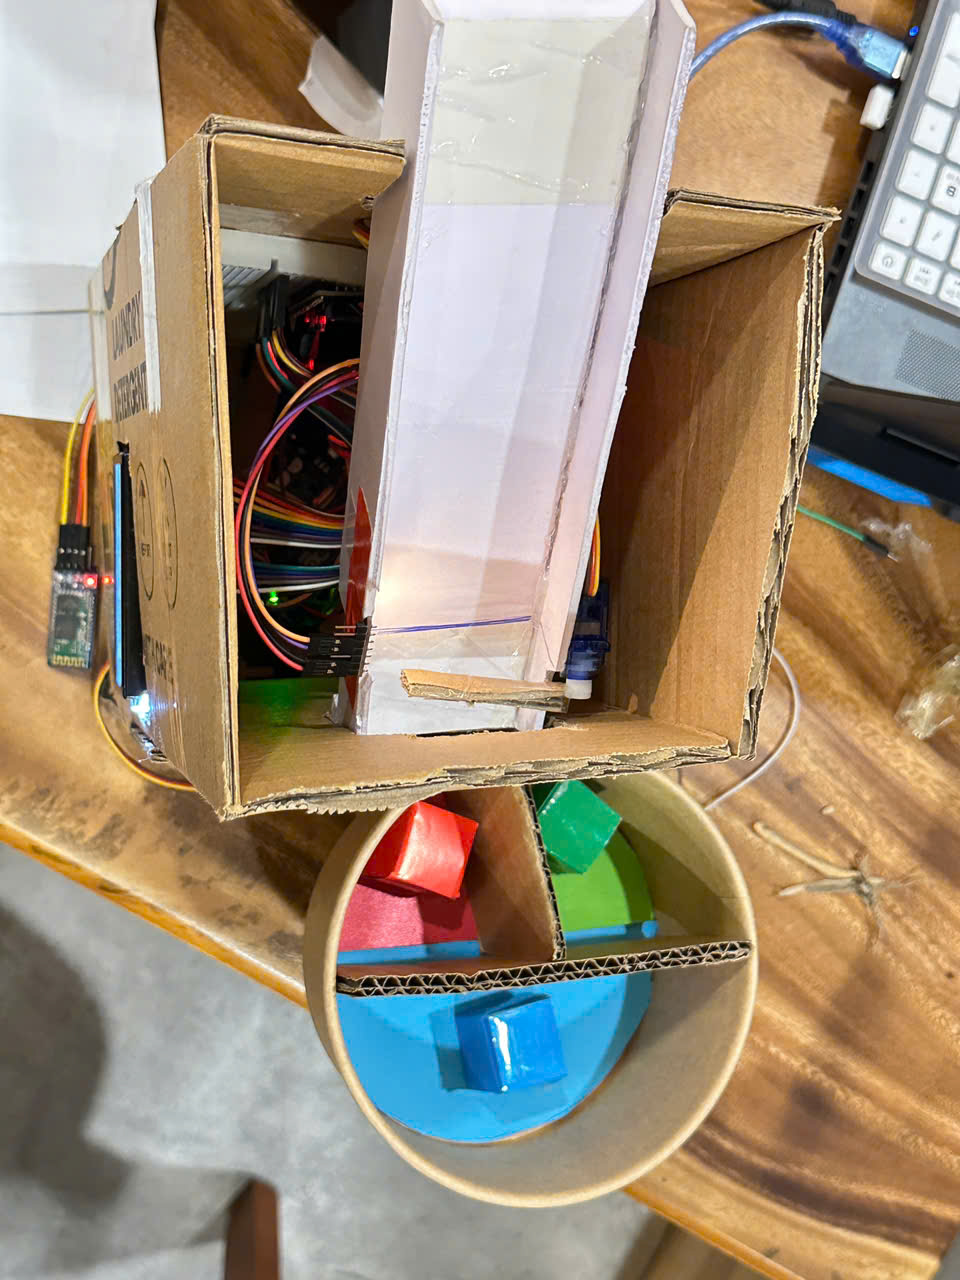
\includegraphics[height=10cm, width=0.7\linewidth\textwidth]{z6445360191681_396b06afdb3631ef00f2b56fdf70380e.jpg}
    \captionof{figure}{Simulation color-based sorting system}
    \label{fig1}
    \end{center}
      \vspace{3em}
\noindent

\begin{center}
    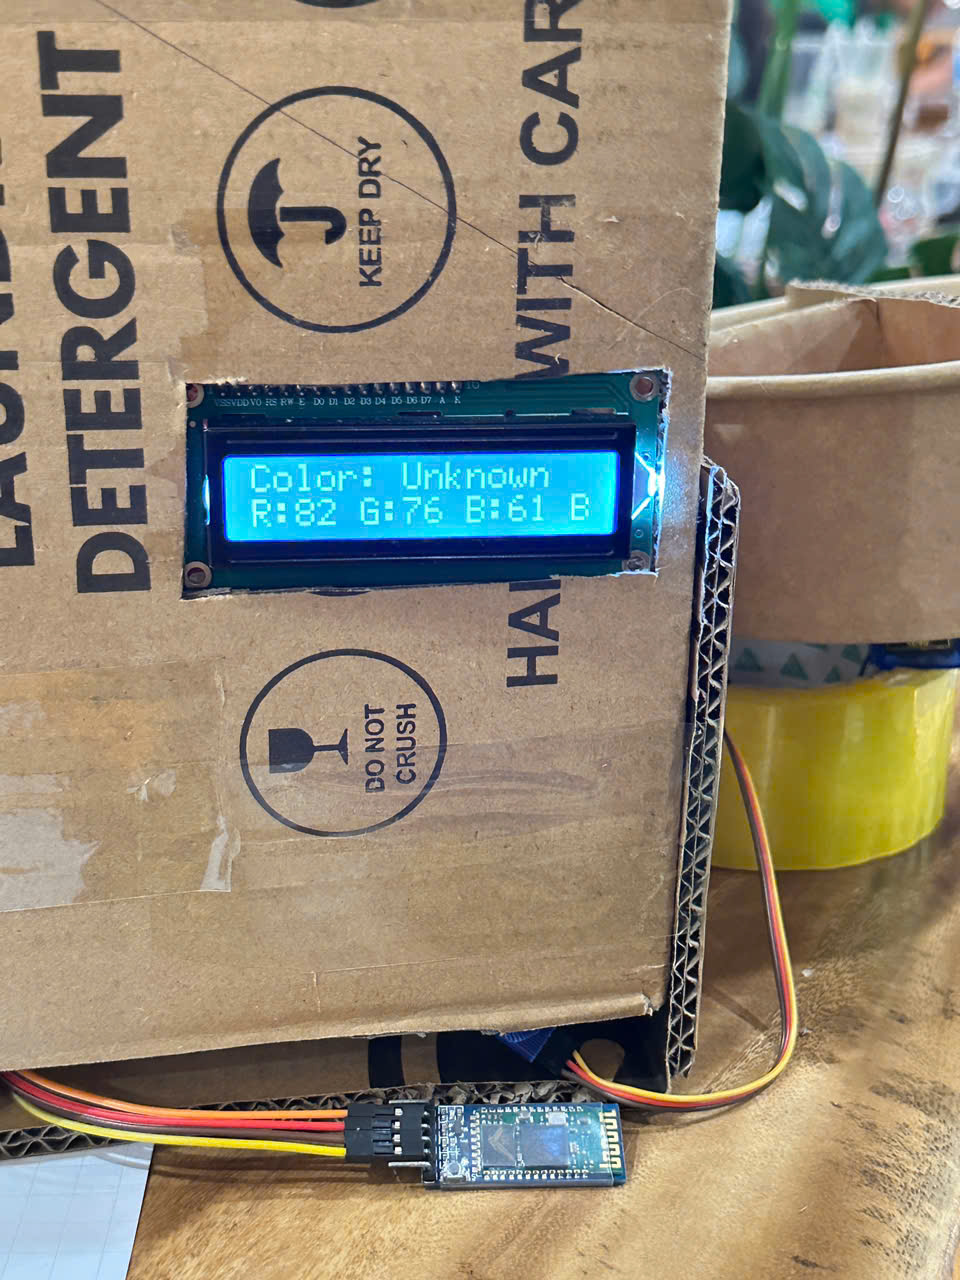
\includegraphics[height=10cm, width=0.7\linewidth\textwidth]{z6445360191814_a188ca7ed7c94401c9256fbc65dc1446.jpg}
    \captionof{figure}{monitor}
    \label{fig1}
    \end{center}
      \vspace{3em}
\noindent
\begin{center}
    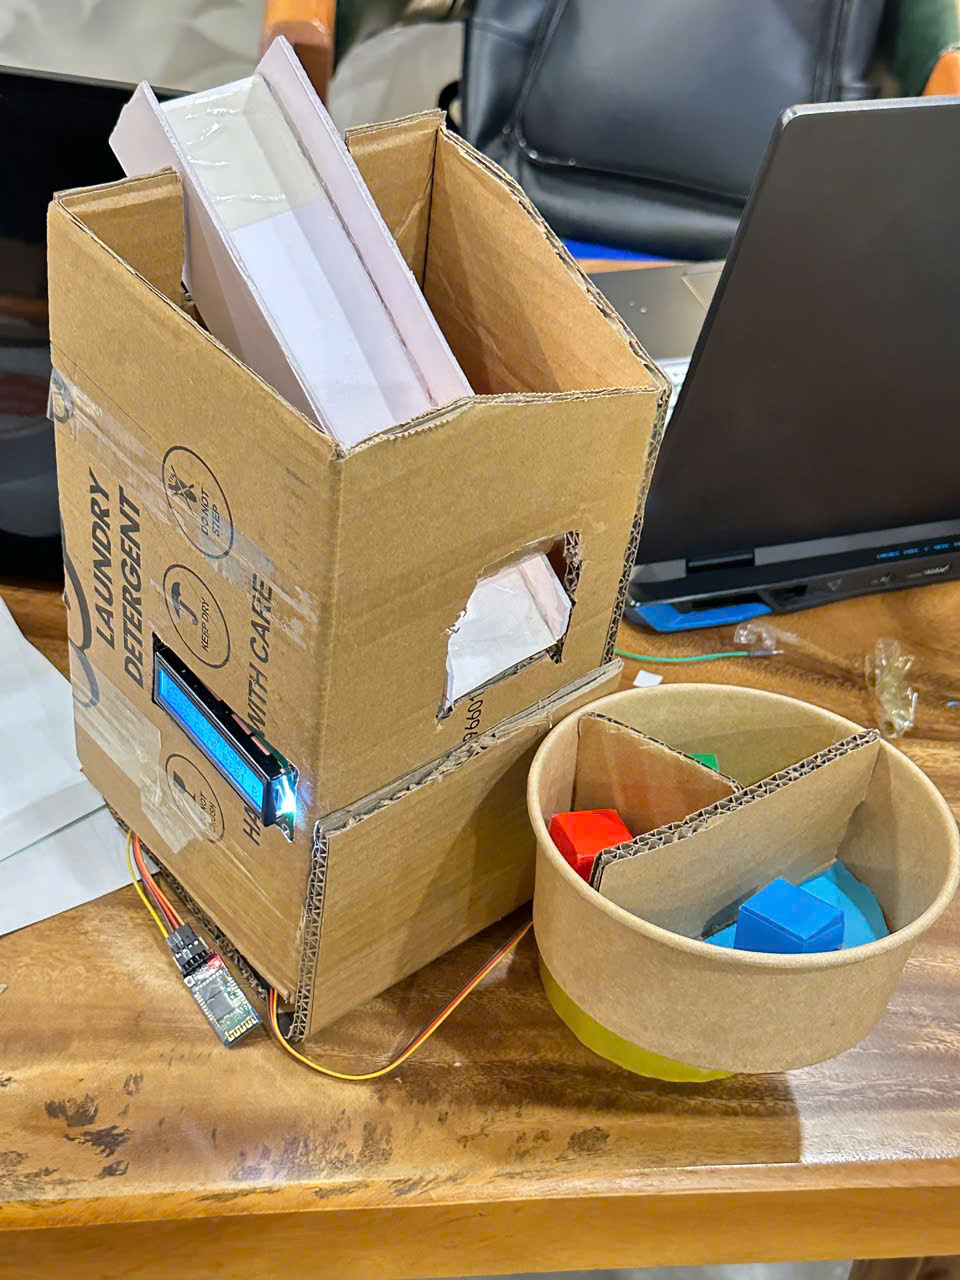
\includegraphics[height=10cm, width=0.7\linewidth\textwidth]{z6445360211195_796fd724118b6b7ee89f1521bd4de894.jpg}
    \captionof{figure}{color-based sorting}
    \label{fig1}
    \end{center}
      \vspace{3em}
\noindent

\subsection{\textbf{Discussion}}
The Smart Color Recognition System represents a significant advancement in automation and color-based task management, delivering substantial benefits while facing certain challenges that need to be addressed. The system integrates advanced technologies, such as the TCS34725 color sensor and Bluetooth connectivity, for real-time monitoring and data collection. It provides accurate RGB values and operational status, enabling users to easily track and adjust the system remotely. Displaying data on the LCD or a mobile device helps reduce errors and ensures precise responses. The automation of servo and buzzer operations minimizes manual intervention, enhances processing efficiency, and lowers the risk of errors in applications like object sorting, which is particularly valuable in industrial, educational, or research contexts.

\section{Conclusion}

The Color-Based Object Sorting Machine represents a significant advancement in automating object classification, delivering a reliable and efficient solution to challenges posed by traditional sorting methods. Through the integration of the TCS34725 color sensor, Arduino Uno Rev3 microcontroller, and supporting components like the servo motor and Bluetooth module, the system achieves precise color-based sorting with minimal human intervention. Testing and implementation have shown its ability to reduce errors, increase throughput, and enhance operational efficiency in practical settings such as recycling facilities, manufacturing workshops, and quality control environments. The real-time feedback via the LCD and remote monitoring through the mobile application further underscore its practicality and user-friendly design, earning positive responses for its consistency and ease of use.

This project not only addresses the inefficiencies of manual and rudimentary sorting systems but also aligns with the broader push toward scalable, technology-driven industrial processes. Its adaptability across small-scale and larger operations highlights its versatility, while its success reinforces the value of IoT-based innovations in modern automation. Moving forward, opportunities to enhance the system include expanding connectivity with Wi-Fi for broader reach and exploring adaptive algorithms to refine sorting accuracy over time. These developments could elevate its performance, positioning the Color-Based Object Sorting Machine as a forward-thinking tool in the evolving landscape of industrial automation. Ultimately, this work demonstrates how targeted technological solutions can drive precision, efficiency, and sustainability in real-world applications.

\begin{table}[htbp]
	\centering
	\caption{Author's contribution}
	\label{tab:my_label}
	\begin{tabular}{|c|c|c|c|c|}
		\hline
		\#&  Student ID &  Student Name &  Tasks & Contribution\\
		\hline
		1&  SE181760&  Nguyen Tuan Tu& Program Bluetooth, Servo Moto, LCD with I2C, Buzzer, design, Write report and prepare Presentation& 25\%\\
		\hline
		2&  SE184970&  Nguyen Tien Dat& System Model and Block Diagram, Programing Flowchart, design and prepare Presentation& 25\%\\
		\hline
		3&  SE185022&  Tran Hoang Tin& Program Arduino, TSC34725 Color Sensor, Software Programing, design and prepare Presentation& 25\%\\
		\hline
		4&  SE184132&  Tran Thanh Hoai& Abstract, Introduction, Software Programing, design and prepare Presentation & 25\%\\
		\hline
		\multicolumn{4}{|c|}{Total}& 100\%\\
		\hline
	\end{tabular}    
\end{table}



\bibliographystyle{IEEEtran} 
%use this for IT
\bibliography{Bib_references}
\end{document}
